
\chapter{Haplotype inference across the spectrum of relatedness}

\section{Background}
The estimation of haplotypes from SNP genotypes, commonly referred to as `phasing', is a well studied problem in statistical genetics. Existing approaches can be categorised according to the type of cohort each method is designed to phase, and the level of relatedness between the individuals in that cohort. Much of the recent literature is devoted to phasing so-called \emph{unrelated} individuals, such as cohorts that have been collected in many genome-wide association studies (GWAS). The term \emph{unrelated} used here is not strictly accurate, since the study individuals will share an evolutionary history. Individuals within such cohorts are usually distantly related, although it can be the case that cryptic relatives, which exhibit much closer relationships, can exist within these cohorts \citep{voight2005confounding}. Methods that have been developed for estimating haplotypes in such cohorts take advantage of linkage disequilibrium (LD). Over relatively short regions some individuals will share short stretches of sequence due to shared ancestry in that part of the genome. Another way to describe this is that individuals will share short stretches of sequence identical by descent (IBD). The most accurate methods use hidden Markov models (HMMs) that model local haplotype sharing between individuals \citep{stephens2001new, delaneau2013}.

Some of the methods designed for unrelated individuals can also handle mother-father-child trios and parent-child duos  \citep{marchini2006comparison, browning2009unified,delaneau2011linear,delaneau2013, williams2012phasing}. Phasing of such small families is relatively easy since the close family relationships place constraints on the underlying haplotypes, substantially reducing the amount of phase information that needs to be determined. Methods also exist for phasing more complex pedigrees, typically as part of more general pedigree analysis software \citep{lange2013mendel,sobel1996descent,abecasis2002merlin,gudbjartsson2000allegro}.  Whilst accurate, these methods are difficult to incorporate into pre-phasing and imputation pipelines that are now a standard part of genome-wide association studies and meta-analyses~\citep{howie2012fast}. 

The task of phasing in isolated populations is some what of a special case, as individuals from such populations exhibit much higher levels of relatedness. Isolated populations arise when a sub-population is isolated from the main population, which increases the degree of endogamy or within population marriage. This has the effect of reducing the effective population size, reduces genetic diversity and creates `long range' LD between sites in the genome. The reduced population size increases the chance that individuals share a very recent common ancestor, say between 1-10 generations ago. When comparing any two individuals from such populations we would expect to observe that they will share much longer stretches of sequence identically by descent (IBD) than a pair of unrelated individuals from a  non-isolated population.  These long IBD stretches can be exploited to infer very accurate haplotypes, an idea originally proposed by \cite{kong2008detection} who applied it to a large sample from the rather unique Icelandic population with high quality results.

A related problem to phasing is the detection of recombination events. Accurate detection of recombination events in a meiosis is important for the study of fine scale recombination, investigating the association between recombination rates and genetic variation, as well as other covariates and for the creation of genetic maps.  A duo or trio is usually insufficient to detect recombination events, as phasing with Mendel rules produces the haplotypes transmitted from the parent to the child, rather than the true parental haplotypes.  While this is sufficiently accurate for many applications, such as construction of haplotype reference sets~\citep{InternationalHapMapConsortium:2005cu} for imputation~\citep{marchini2010genotype}, it is clearly not useful for studying recombination.  

Recombination events can be inferred from a three generation pedigree since accurate phasing of both parents (via the grandparental genotypes) allows detection of recombination events in their children.  Alternatively, nuclear families with $>2$ children can be used to identify recombination events by examining differences in the transmitted haplotypes between siblings.  This was the approach used to create the deCODE family based map~\citep{kong2002} from families sampled from the Icelandic population, as well as by \cite{coop2008high} using individuals from a Hutterite population.  As genotyping error complicates such approaches, Coop applied ad-hoc filtering to detect clusters of unlikely recombination events and achieved good results.  Both of these studies exploit pedigrees that are informative about recombination.  In the absence of such data, we need to be able to very accurately phase the parental haplotypes using information from the wider population. This was recently achieved using a long-range phasing approach to obtain the true parental haplotypes (and hence recombination events) in Icelandic individuals~\citep{kong2010fine}.  

It would appear that different phasing tools (or a mixture thereof) should be applied depending on the demography of a cohort. In this chapter we give an overview of the popular methods for phasing cohorts of unrelated individuals, individuals that exhibit large tracts of IBD sharing (long range phasing) and the Lander-Green algorithm for extended pedigrees.  We also introduce our own technique for incorporating extended pedigree information into haplotypes that were inferred using methods for unrelated individuals, with the aim of overcoming the limitations of traditional pedigree approaches.  This method, called the duoHMM, ensures haplotypes are consistent with pedigree structure and can also detect recombination events. In chapter 4 we evaluate the accuracy of all of these approaches on real and simulated data. 

\subsection{The switch error metric}
Given a set of ``true'' validation haplotypes and some haplotypes inferred via a method, we require a sensible metric to evaluate the accuracy of each of our inferred haplotype sets.  Switch error (SE) rate was introduced by \cite{Lin:2002hh}  and has become the defacto metric for phasing evaluations~\citep{stephens2003comparison}.  It is defined as the proportion of adjacent heterozygote sites that are incorrectly aligned, each of these incorrect alignments is referred to as a switch error. We can think of this as the number of times an inferred haplotype needs to be switched (or flipped) so that it matches the true haplotype.  Figure~\ref{chap3:switcherror} (top) illustrates this idea showing an inferred haplotype which has two switch errors and six heterozygous sites resulting in a switch error rate of $\frac{2}{6-1}=0.4$

\begin{figure}[h]
  \begin{center} 
    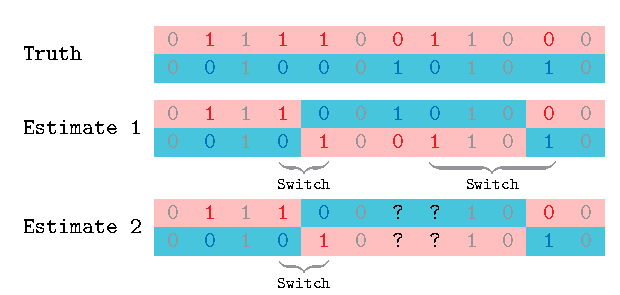
\includegraphics[width=\textwidth]{chap3figs/switcherror}
    \caption[Examples of the switch error metric]{Examples of the switch error metric.  The true underlying parental chromosomes are in pink and light blue with heterozygous sites (the sites of interest) highlighted in red and dark blue.   Estimate 1 has two switch errors present meaning that we would need to flip the estimated haplotype twice to arrive at the true underlying haplotype.  Estimate 2 is only partially phased (which can be the case with SLRP's output) and whilst there is a switch error between the heterozygous sites flanking the unphased region, we ignore this for comparison purposes since the algorithm was not attempting to align these sites correctly. \label{chap3:switcherror}}
  \end{center} 
\end{figure}
\clearpage
In this chapter we describe methods that are not capable of resolving every heterozygous site, the Lander-Green (LG) algorithm and SLRP, this complicates the evaluation of switch error rates. There are two types of missingness to consider here.  The first is where a heterozygous site is left unphased because that locus is heterozygous throughout a pedigree (LG) or throughout an IBD cluster (SLRP).  In this case the flanking heterozygote sites should still be aligned correctly if the method has not made an error and the IBD status has not changed.  We simply ignore such sites when calculating switch errors. The second case only occurs with SLRP's estimated haplotypes.  A chromosome may have large regions which are left completely unphased due to a lack of IBD sharing.  The flanking heterozygous sites of such a region will be phased at random, and we ignore switch errors in such cases essentially treating the phasing IBD blocks as mini-chromosomes. Figure~\ref{chap3:switcherror} (bottom) gives a toy example of two phased IBD chunks separated by an unphased region and how we calculate switch errors in such a situation.


\subsection{Statistical framework}
After genotype calling on microarrays similar to that described in the previous chapter, we are left with a vector of  genotypes at $L$ markers across a chromosome for individuals $i = 1...N$, that is $G_i = \{G_{i1},...,G_{iL}\}$.  We assume bi-allelic variants  so $G_{il}\in \{0,1,2\}$ is the sum of the two inherited parental alleles (coded as 0/1)  at the $l$th SNP.   Throughout this chapter, we denote the underlying pair of haplotypes (or diplotype) for an individual as $(h^1,h^2)$ where $h^1$ and $h^2$ are vectors of binary variables of length $L$ such that $G_{il} = h_{il}^1 + h_{il}^2$. Generally speaking, we typically wish to obtain the posterior distribution of an individual's haplotypes, conditional on their genotypes as well as other genotypes in a cohort (or within the same pedigree), that is $P(h^1,h^2|G_1,\ldots, G_N)$. All of the methods described in this chapter utilise HMMs of varying structure where the hidden states correspond to some relatedness between individuals in the cohort.  Depending on the sample this relatedness ranges from very distant (linkage disequilibrium) to very recent (explicit pedigree relationships).

\subsection{Hidden Markov Models}
Every model described in this chapter utilises some form of HMM to estimate haplotypes.  We briefly cover some key concepts  following the well known tutorial given by \cite{rabiner1989tutorial}.  Phasing applications typically involve discrete state Markov chains with inhomogeneous transition probabilities. We have a sequence of random states $Z=\{Z_1,\ldots,Z_L\}$ that follow the Markov property with transition probabilities that vary with position $l$. We do not observe these states directly, but rather some emitted variables, $X=\{X_1,\ldots,X_L\}$.  The distribution of $X_l$ depends on the hidden state $Z_l$. Hence we have two components for a HMM, the transition probabilities that describe the Markov process; $P(Z_1)$ and $P(Z_{l+1}|Z_l)$ as well as the conditional distribution of the observed variable $X$ given the state, $P(X|Z)$ (often referred to as the emission distribution).  The likelihood of some observed data is then
$$P(X) = \sum_Z P(Z_1) \prod_{i=2}^L P(Z_l|Z_{l-1}) \prod_{i=1}^L P(X_l|Z_l) $$
where we are summing over every possible state sequence $Z$.  Performing this calculation na\"{\i}vely is clearly intractable for any problem of moderate size, but can be found via a dynamic programming technique known as the Forward-Backward algorithm.  

The forward variable is defined as:
$$\alpha_l(k) = P(X_1,\ldots,X_l,Z_l=k)$$
which can be calculated by induction with initialisation step
$$\alpha_1(k) =   P(X_1|Z_1=k) P(Z_1=k)$$
and induction step 
$$\alpha_{l+1}(k) = P(X_{l+1}|Z_{l+1}=k) \sum_{k'=1}^K \alpha_l(k') P(Z_{l+1}=k|Z_l=k')$$
then $\sum_{k=1}^K \alpha_{L}(k)$ is the likelihood of the observed sequence.  Similarly we have the backward variable:
$$\beta_l(k) = P(X_{l+1},\ldots,X_L|Z_l=k)$$
which is calculated by induction with with initialisation step
$$\beta_L(k) = 1$$
and induction step 
$$\beta_l(k)  =  \sum_{k'=1}^K P(X_{l+1}|Z_{l+1}=k') \beta_{l+1}(k')P(Z_{l+1}=k'|Z_l=k)$$
Typically we are interested in the posterior distribution of the sequence $Z$ given the observed data $X$, that is $P(Z|X)$.  The forward and backward variables allow us to calculate the posterior probabilities of states at a specific location $l$:
$$P(Z_l=k|X_1,\ldots,X_L) \propto \alpha_l(k)\beta_l(k)$$
alternatively, we may be interested in the most likely state sequence rather than just the most likely state at one specific position.  The most likely state sequence can be found via the Viterbi algorithm which involves calculating the variable:
$$\delta_l(k) = \max_{k_1,\ldots,k_{l-1}} P(Z_1,\ldots,Z_l=k,X_1,\ldots,X_l)$$
which is the most likely state sequence leading up to state $k$ at time $l$.  This can be calculated recursively similarly to the forward variable with initialisation:
$$\delta_1(k) =   P(X_1|Z_1=k) P(Z_1=k)$$
and induction:
$$\delta_{l+1}(k) = P(X_{l+1}|Z_{l+1}=k) \max_{k'} \left(  \delta_l(k') P(Z_{l+1}=k|Z_l=k') \right)$$
in addition to $\delta$, we require the value of $k'$ that maximises this term for each $k$ and $l+1$.  Again using induction we have initialisation
$$\psi_1(k)=0$$
and induction step
$$\psi_l(k)=\argmax_{k'} \left(  \delta_l(k') P(Z_{l+1}=k|Z_l=k') \right).$$
We can then infer the most likely state sequence, $\{\hat{Z}_1,\ldots,\hat{Z}_L\}$ with initialisation
$$\hat{Z}_L = \argmax_{k}(\delta_T(k))$$
and induction
$$\hat{Z}_l = \psi_{l+1}( \hat{Z}_{l+1})).$$
Rather than obtain the most likely state sequence, we may wish to sample a state sequence from the distribution $P(Z_1,\ldots,Z_L|X)$.  This is an effective way of taking into account the uncertainty in the estimated sequence and is of use in the Markov Chain Monte Carlo (MCMC) routines described later in this chapter. To sample a sequence, we only require the calculation of the forward variable.  We first sample a state at position $L$ from 
$$P(\hat{Z}_L=k|X)  \propto \alpha_L(k)$$
and then recurse backwards sampling at each $l$:
$$P(\hat{Z}_l=k|\hat{Z}_{l+1}=k',X) \propto \alpha_l(k) P(\hat{Z}_l=k|\hat{Z}_{l+1}=k')$$
terminating at $l=1$.  

It is important to note that the complexity of calculating the forward, backward and Viterbi variables is $O(LK^2)$.  This means computation will scale well with the number of markers (which can be very large in phasing applications) but will rapidly become intractable as the state space increases. Many of the advances in phasing described in this chapter involve innovative ways of reducing the state space whilst maintaining accuracy.


\section{Methods for nominally unrelated individuals}
\label{chap3:unrelated}
\subsection{The Li and Stephens Model for Linkage Disequilibrium}
\label{chap3:liandstephens}
The Li and Stephens model~\citep{li2003model} is now a classic approximate model for linkage disequilibrium that was originally proposed to perform inference on recombination rates across a chromosome.  It forms the basis for various phasing (and associated imputation) software such as IMPUTE1~\citep{marchini2007new}, IMPUTE2~\citep{howie2009flexible}, MaCH~\citep{li2010mach}, HAPI-UR~\citep{williams2012phasing} and both versions of SHAPEIT~\citep{delaneau2013,delaneau2011linear}.

Consider the case where we have $K$ known haplotypes sampled from the population, $H =\{H_1 \ldots H_K\}$ where $H_k=\{H_{k1},\ldots,H_{kL}\}$.  The $K+1$ sampled haplotype, $h=\{h_1,\ldots,h_L\}$, is modelled as a mosaic of the $K$ already sampled haplotypes, along with some sporadic allelic differences due to mutation events. Put another way, haplotype $h$ ``copies from'' different haplotypes in the sample at different regions along the chromosome. We use $Z_l \in \{1,\ldots,K\}$  to denote which of the $K$ haplotypes is being copied from at position $l$.  This forms a Hidden Markov Model with transition probabilities varying according to recombination rates where $h$ is the observed variable and $Z$ are the hidden states of the chain. The initial state is distributed uniformly:
$$P(Z_1=k) = 1/K$$
at subsequent markers, state transitions are
\[ P(Z_{l+1}=k|Z_l=k')  = \left\{ 
  \begin{array}{l l}
    \frac{1-\exp(-\frac{\rho_l}{K})}{K} & \quad k \neq k'\\
    \exp(-\frac{\rho_l}{K}) + \frac{1-\exp(-\frac{\rho_l}{K})}{K} & \quad k = k'
  \end{array}  \label{chap3:listephentrans}
  \right.\]
where $\rho_l = 4N_er_l$ and $r_l$ is the genetic distance (in Morgans) between sites $l$ and $l+1$. This transition matrix has two intuitively sensible properties. First, when the distance between markers is small, then those markers are highly likely to copy the same chromosome. Second, as the sample size $K$ increases, the chance of a change in copying state decreases, meaning longer haplotype chunks tend to me copied.

Mutation events are handled by the emission distribution:
\begin{equation}
%\[ 
P(h_l= A_{kl}|Z_l=k) = \left\{ 
  \begin{array}{l l}
    1-\frac{\theta}{2(\theta+K)}               & \quad h_l = A_{kl}  \\
    \frac{\theta}{2(\theta+K)}      & \quad h_l \neq A_{kl} 
  \end{array}  
\right.
%\]
\label{chap3:listephenmut}
\end{equation}
where $A_{kl}$ denotes the allele carried by the $k$th haplotype at site $l$. The parameter  $\theta = (\sum_{m=1}^{K-1} \frac{1}{m})^{-1}$ controls the rate of mutation.  The intuition behind this choice of $\theta$ is that $\theta \times (\sum_{m=1}^{K-1} \frac{1}{m})$ is the expected number of mutations events at a single site for $K$ individuals, the model sets this expectation to 1 and solves for $\theta$.

The Li and Stephens model has the desirable property that the length and fidelity of haplotypes copied increases with $K$, reflecting the fact that as sample size increases, individuals will tend to share larger and more similar haplotypes. It also has the crucial benefit of allowing tractable inference using well developed HMM inference machinery.

\subsubsection{Inference with the Li and Stephens Model}
The likelihood for an individual haplotype is
$$P(h_1,\ldots, h_L|H) = \sum_Z \prod_{l=1}^L P(h_l|Z_l) P(Z_1) \prod_{l=2}^L  P(Z_l|Z_{l-1})$$
here we need to integrate over every possible configuration of copying sequences ($Z$), which is a standard operation for HMMs using the Forward-Backward algorithm. Whilst in general inference on a HMM with $K$ states will have computational cost of  
$O(LK^2)$, inference on the Li and Stephens model can be performed in $O(LK)$ due to the probability of a change in copying state being the same regardless of which states are being transitioned between.  For example if we take the standard HMM forward variable:
$$\alpha_l(k) = P(h_1,\ldots,h_l,Z_l=k)$$
which is calculated by induction with initialisation step
$$\alpha_1(k) = \frac{1}{K} P(h_1|Z_1=k)$$
and induction step 
\begin{eqnarray*}
\alpha_{l+1}(k) & = & P(h_{l+1}|Z_{l+1}=k) \sum_{k'=1}^K \alpha_l(k')P(Z_{l+1}=k|Z_l=k') \\
					&=& P(h_{l+1}|Z_{l+1}=k)\left( \exp(-\frac{\rho_l}{K})\alpha_l(k) + \frac{1-\exp(-\frac{\rho_l}{K})}{K}\sum_{k'=1}^K\alpha_l(k')\right)
\end{eqnarray*}
the right term of the summation is the same for all $k$ and hence only needs to be evaluated once per site so computation scales with $O(LK)$ complexity.  For the same reason, calculation of the backward variable and the Viterbi algorithm are both $O(LK)$. Hence the Li and Stephens model offers a powerful tool for the tractable analysis of genetic data where both the sample size $K$ and number of sites $L$ can be very large.

%% Similarly for the backward variable:
%% $$\beta_l(k) = P(h_{l+1},\ldots,h_l|Z_l=k,\rho)$$
%% which is calculated by induction with with intialisation step
%% $$\beta_L(k) = 1$$
%% and induction step 
%% \begin{eqnarray*}
%% \beta_l(k) & = & \sum_{k'=1}^K P(h_{l+1}|Z_{l+1}=k') \beta_{l+1}(k')P(Z_{l+1}=k'|Z_l=k) \\
%% &=&  \frac{1-\exp(\frac{\rho_l}{K})}{K}\sum_{k'=1}^KP(h_{l+1}|Z_{l+1}=k')\beta_{l+1}(k') + \exp(-\frac{\rho_l}{K})P(h_{l+1}|Z_{l+1}=k)\beta_{l+1}(k)
%% \end{eqnarray*}
%% Again we can save computation  by only computing the left term of the summation once. Inference on HMMs revolves around these two calculations as well as the Viterbi algorithm (which is similar to the forward variable calculation) 


\subsection{Phasing with the Li and Stephens Model}
\label{chap3:LSphase}
The previous section gave us a useful model for observed \emph{haplotypes} in a sample, but in practice we observe \emph{genotypes}. IMPUTE1 and IMPUTE2 extended the Li and Stephens model to genotype data for the purposes of phasing and genotype imputation from haplotype reference panels (a closely related problem).  We summarise the general approach of this extension here.


\begin{figure}[h]
  \begin{center} 
    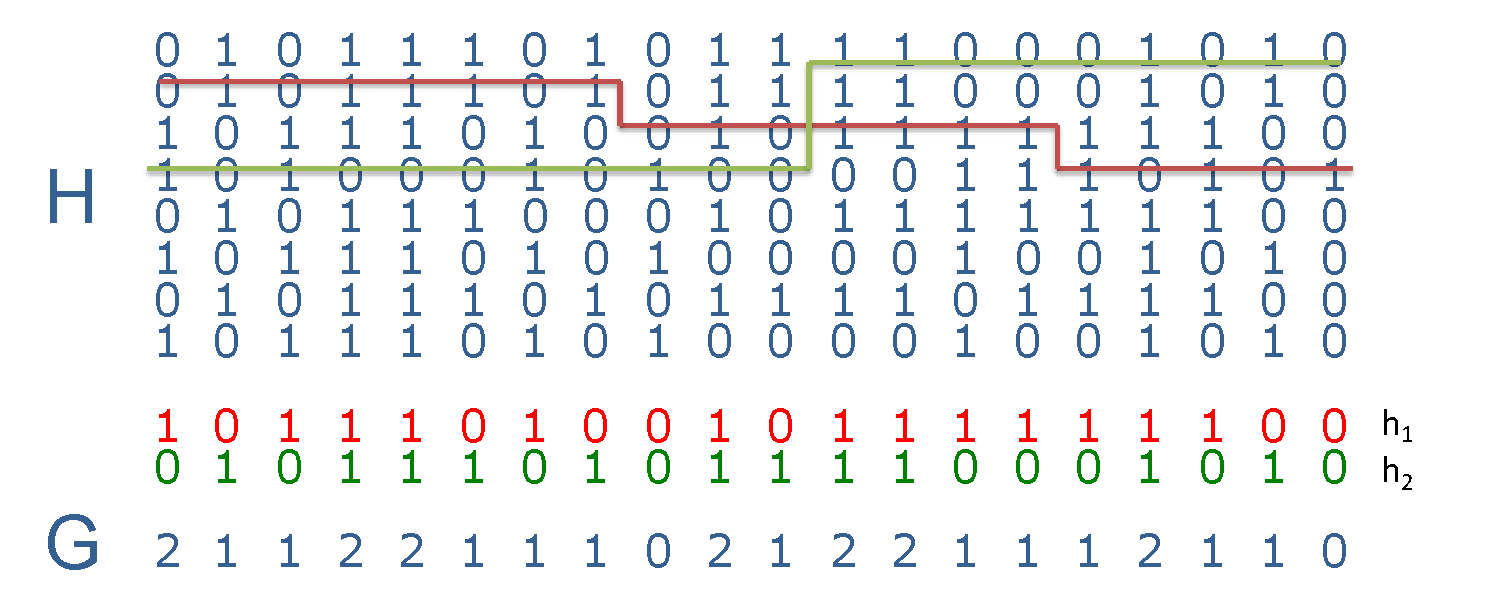
\includegraphics[width=\textwidth]{chap3figs/haplotype_path}
    \caption[Inferring haplotypes with the Li and Stephens Model]{An example of a pair of copying paths for the diploid Li and Stephens model used to infer an individual's underlying haplotypes, $(h_1,h_2)$, from that individual's genotype data $G$.  The individual's haplotypes are inferred as a mosaic of other \emph{conditioning haplotypes}, $H$ in the population.   \label{chap3:happath}}
  \end{center} 
\end{figure}

Given a set of conditioning haplotypes, $H$, an individual's diplotype, $(h^1,h^2)$, originates from a pair of sequences of hidden states $(Z^1,Z^2)$ where $(Z^1_l,Z^2_l)\in\{1\ldots K\}$ denote which conditioning haplotypes  an individual's haplotype  pair is copying from at site $l$.  Using the model defined in the previous section and assuming an individual's haplotypes are independent of one another, we now have a Hidden Markov Model with $K^2$ states (every possible pairing of copying states). 

The initial state probabilities for Markov chain are:
$$P(Z_1^1=k_1,Z_1^2=k_2) = 1/K^2$$
and the transition probabilities are:
\small
\[ P(Z_{l+1}^1=k_1,Z_{l+1}^2=k_2 | Z_l^1=k_1',Z_l^2=k_2') = \left\{ 
  \begin{array}{l l}
    \left( \exp(-\frac{\rho_l}{K}) + \frac{1-\exp(-\frac{\rho_l}{K})}{K} \right) ^2 & \quad k_1=k_1',~k_2=k_2'\\
    \left( \frac{1-\exp(-\frac{\rho_l}{K})}{K} \right) \left( \exp(-\frac{\rho_l}{K}) + \frac{1-\exp(-\frac{\rho_l}{K})}{K} \right) & \quad k_1 \neq k_1' \oplus  k_2 \neq k_2'\\
    \left( \frac{1-\exp(-\frac{\rho_l}{K})}{K} \right)^2 & \quad k_1\neq k_1',~k_2\neq k_2'\\
  \end{array} \right.\label{chap3:jump}\] 
\normalsize
these probabilities correspond to 0, 1 and 2 ``jumps'' between which conditioning haplotypes an individual's diplotype is copying from. Figure~\ref{chap3:happath} provides an example of a genotype and corresponding paths through the conditioning haplotypes. 

 Given an observed genotype $G_{il}$ at position $l$ and hidden states $(Z^1_l,Z^2_l)$, the emission distribution $P(G_{il}|Z^1_l,Z^2_l)$ for each possible combination is: 
\vspace{10pt}
\begin{center}
\begin{tabular}{|c|l|cccc|}
  \hline
  &  &\multicolumn{4}{c|}{$G_{il}$}\\
  &  & 0 & 1 & 2 & Missing \\ 
  \hline
  \multirow{3}{*}{$h_{Z^1_l}+h_{Z^2_l}$} & 0 & $(1-\lambda)^2$ & $2\lambda(1-\lambda)$ & $\lambda^2$ & 1.0 \\ 
                                     & 1 & $2\lambda(1-\lambda)$ & $\lambda^2 + (1-\lambda)^2$ & $2\lambda(1-\lambda)$  & 1.0 \\ 
                                     & 2 & $\lambda^2$ &$2\lambda(1-\lambda)$ &$(1-\lambda)^2$ & 1.0 \\
   \hline
\end{tabular}
\end{center}
\vspace{10pt}
where $\lambda=\frac{\theta}{2(\theta+K)}$, the mutation probability seen in the Li and Stephens model (Equation~\ref{chap3:listephenmut}). Note that this model easily accommodates missing genotypes by placing a flat likelihood across also possible genotype values. The likelihood for an observed genotype vector is then
\begin{equation}
P(G_i|H) = \sum_{Z^1,Z^2} ~\prod_{l=1}^L  P(Z_{l}^1,Z_{l}^2) \prod_{l=1}^L P(G_{il}|Z^1_l,Z^2_l).
\label{chap3:impute2lik}
\end{equation}
here we are summing over all possible unobserved paths ($Z_1,Z_2$). 

 We are primarily interested in the posterior distribution of an individual's haplotypes conditional on all other information, $P(h_1,h_2|G_i,H)$ which in turn is determined by the pair of copying paths $P(Z_1,Z_2|G_i,H)$. The complexity of our state space has increased substantially compared to the haploid model described previously.  Consider the calculation for the forward variable of this model:
$$\alpha_l(k_1,k_2) = P(G_{i1}\ldots G_{il+1},Z_{l+1}^1=k_1,Z_{l+1}^2=k_2|H)$$
with initialisation step:
$$\alpha_1(k_1,k_2) = \frac{1}{K^2} \times (G_{il}|Z^1_l=k_1,Z^2_l=k_2)$$
and induction step:
\begin{eqnarray*}
  \alpha_{l+1}(k_1,k_2) & = & P(G_{il}|Z^1_l=k_1,Z^2_l=k_2) \times\\
  &&\Bigg[  \left(\exp(-\frac{\rho_l}{K}) + \frac{1-\exp(-\frac{\rho_l}{K})}{K}\right)^2 \alpha_l(k_1,k_2)\\
    && + \left( \frac{1-\exp(-\frac{\rho_l}{K})}{K} \right) \left( \exp(-\frac{\rho_l}{K}) + \frac{1-\exp(-\frac{\rho_l}{K})}{K} \right) \left( \sum_{k'=1}^K \alpha_l(k',k_2) + \sum_{k'=1}^K \alpha_l(k_1,k')\right)\\
    && +  \left( \frac{1-\exp(-\frac{\rho_l}{K})}{K} \right)^2 \left( \sum_{k_1'=1}^K \sum_{k_2'=1}^K \alpha_l(k_1',k_2') \right) \Bigg]
\end{eqnarray*}
the middle summations require $2K^2$ operations to calculate across all pairs of $(k_1,k_2$). \cite{scheet2006fast} provide derivations which exploit the symmetry $ \alpha_{l}(k_1,k_2) =  \alpha_{l}(k_2,k_1)$ to avoid redundant computations, approximately halving the computational burden. This is an important implementational detail but we exclude it for clarity. The essential point is that inference procedures for HMMs on genotype data under the Li and Stephens model now scale quadratically with the size of $H$.

We have described the model assuming that conditioning haplotypes were known, we could possibly use a reference panel of haplotypes such as those available from the 1000 Genomes Project, which was in fact how IMPUTE1 functioned.  However results from the development of IMPUTE2 showed that phasing using in-sample conditioning haplotypes was more effective than the reference panel only approach. Hence using conditioning haplotypes present in the sample is preferable, but of course these are unknown, so we need to integrate over this uncertainty. This can be achieved via an MCMC approach.

Given a sample of $N$ genotyped individuals, $G = G_1\ldots G_N$, we wish to infer each individual's diplotypes ($2N$ haplotypes), $H = \{H_1,\ldots,H_{2N}\}$.  We can initialise the haplotypes of all individuals by randomly assigning phase at all heterozygous sites.  We can then iterate over each individual, sampling a diplotype from $P(h^1,h^2|G_i,H \setminus (H_{2i-1},H_{2i}))$.  This process is repeated for a set number of iterations.  Finally we can either run the Viterbi algorithm to find the most likely haplotypes for an individual or take the most likely diplotype per site $l$. An issue with this approach is that computation scales quadratically with sample size $N$ meaning the method rapidly becomes intractable with increasing sample size.  This problem can be circumvented by only conditioning on a subset of size $K<2(N-1)$ of the haplotypes in the sample, constraining computation to $O(LK^2)$.

\subsubsection{Choosing conditioning haplotypes}
We could choose these $K$ conditioning haplotypes at random from the cohort which is the approach used by MaCH.  Alternatively, we could try to choose conditioning haplotypes such that they are likely to be ``copied'' from by the individual being phased. This is the ``surrogate-family'' approach introduced by IMPUTE2. In this approach, the Hamming distance between the individual's previously sampled haplotypes $H_i=(h^1_i,h^2_i)$ and all other $2(N-1)$ haplotypes present in the sample is calculated. The Hamming distance is simply the sum of alleles that are different across a region.  The $K$ haplotypes with the smallest distance measures, $H^{*}=\{H_1,\ldots,H_K\}$, are used as the conditioning set for individual $i$.  We then work with the posterior $P(h_1,h_2|G_i,H^{*})$  which restrains the HMM computations to $O(K^2L)$ complexity. Since an individual's closest ancestors in a sample will vary across a chromosome, it was recommended to run IMPUTE2 on chunks of several Mb so that a different $H^{*}$ would be used in different genomic regions.

This can be thought of as conditioning on all haplotypes in the cohort in a very crude manner, as all haplotypes are still being compared.  Since the distance calculations involve comparing each individual to all $N$ samples in a cohort at all loci, they have $O(N^2L)$ complexity.  However because these operations are very rapid, the HMM calculations dominate computation for $N<10000$.  As sample sizes increase to tens of thousands of individuals, these distance calculations begin to comprise the majority of computation. 

\subsection{The SHAPEIT2 approach}
The Segmented HAPlotype Estimation and Imputation Tool version 2 (SHAPEIT2)~\citep{delaneau2013} is a recently developed method for phasing unrelated individuals. It combines a novel data structure for efficiently representing the space of possible  haplotypes of an individual which was introduced in the original SHAPEIT1~\citep{delaneau2011linear} along with the ``surrogate-family'' conditioning haplotype selection idea introduced by IMPUTE2. The main advantage of this approach over IMPUTE2 is that the HMM calculations  scale \emph{linearly} with the number of conditioning haplotypes, this means computation can performed tractably with larger values of $K$ leading to greater accuracy and less computation time.

An individual's genotype vector $G_i$ can be partitioned into $C$ segments where each segment contains $B$ heterozygous sites.  There will be $2^B$ consistent haplotypes within each of these segments.  The vector $S_l \in \{1\ldots C\}$ denotes which segment contains locus $l$. A haplotype that is consistent with $G_i$ across the chromosome can now be represented as a sequence of labels $X = \{x_1,\ldots,x_L\}$  where $x_l$ is now the label of the segmental haplotype at position $l$.  We allow the label $X$ to change only between segments, that is, when $S_l\neq S_{l+1}$.  Figure~\ref{chap3:s2seg} shows an example of this graph for three segments and $B=2$. A sequence $X$ now uniquely defines a haplotype that is consistent with $G$. 

Furthermore, the sequence $X$ also implies its unique complementary haplotype (to enforce consistent genotypes with $G$), so $X$ in fact implies a diplotype consistent with $G$.  This is the key to SHAPEIT2's linear complexity calculations, inference is now being performed on one haploid path, $X$, rather than a pair of haploid paths as in IMPUTE2.

\begin{figure}
  \begin{center} 
    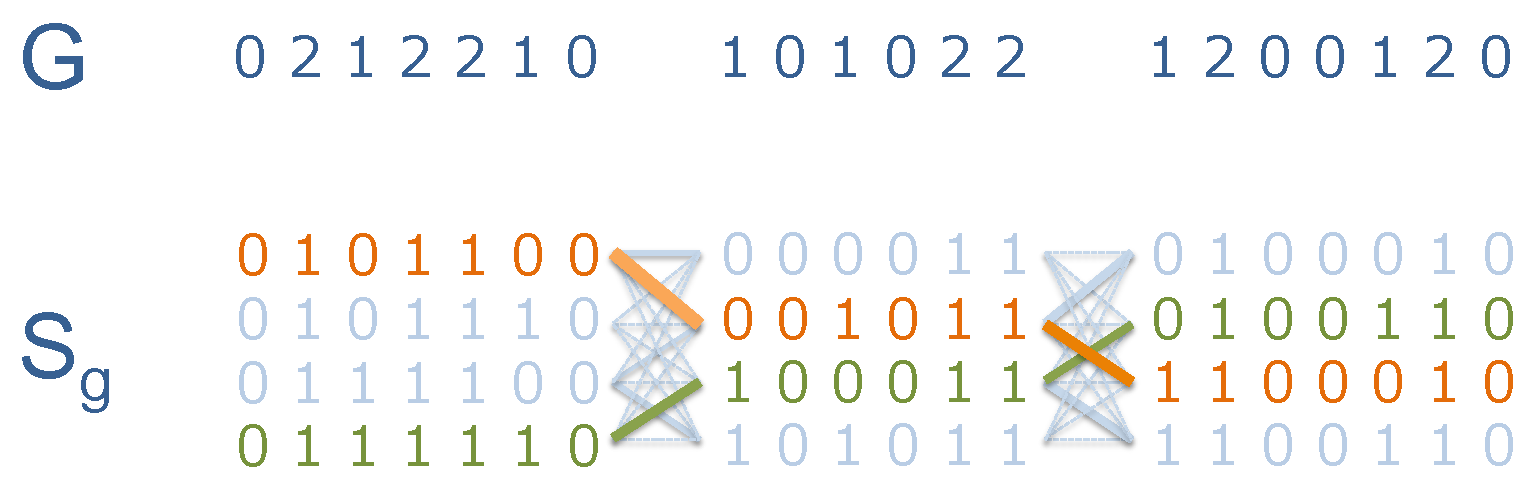
\includegraphics[width=\textwidth]{chap3figs/shapeit_model}
    \caption[The SHAPEIT2 diploid model]{The SHAPEIT2 diploid model, within each segment containing $B=2$ two heterozygous genotypes there are $2^B$ possible haplotypes.  Transitions between different haplotype labels are only possible \emph{between} segments, not within them.  The green and orange colouring labels a pair of paths consistent with the genotype vector.\label{chap3:s2seg}}
  \end{center} 
\end{figure}

This segmentation provides a graph that captures every possible haplotype for an individual, we can weight the edges of this graph using patterns of LD present in the conditioning haplotypes $H$ and the Li and Stephens model. This introduces a second latent variable $Z$,  denoting the haplotype in $H$ being copied from. For a single consistent haplotype, there are now two unobserved sequences, $X$ and $Z$.  Hence we perform inference on the likelihood:

$$P(X,Z|H) = P(X_1|Z_1,H) P(Z_1) \prod_{l=2}^L P(X_l,Z_l|X_{l-1},Z_{l-1},H)$$

We take the same transition probabilities as used in the haploid Li and Stephens model, but with the added restriction that the haplotype label ($X_l$) can only change when positions $l$ and $l-1$ are on different segments.  So when $S_l=S_{l-1}$ then transition probabilities are
\[ P(X_l=i,Z_l=k|X_{l-1}=j,Z_{l-1}=k',H) = \left\{ 
  \begin{array}{l l}
%     P(X_l=i,Z_l=k,H) P(Z_l=k|Z_{l-1}=k')  & \quad i=j\\
    P(Z_l=k|Z_{l-1}=k')  & \quad i=j\\
     0    & \quad  i\neq j\\
  \end{array} \right.\] \label{chap3:listephentrans} 
and when sites are on different segments ($S_l\neq S_{l-1}$) any transition is possible so
%$$ p(X_l=i,Z_l=k|X_{l-1}=j,Z_{l-1}=k',H) =  P(X_l=i,Z_l=k,H) P(Z_l=k|Z_{l-1}=k') $$
$$ p(X_l=i,Z_l=k|X_{l-1}=j,Z_{l-1}=k',H) =  P(Z_l=k|Z_{l-1}=k') $$
The emission probability is also the same as the Li and Stephens mutation model (Equation~\ref{chap3:listephenmut}):
\[ P(X_l=i|Z_l=k,H)  = \left\{ 
  \begin{array}{l l}
    \frac{\theta}{2(\theta+K)}               & \quad H_{kl} \neq A_{il}\\
    1-\frac{\theta}{2(\theta+K)}      & \quad H_{kl} = A_{il}
  \end{array}  
\right.\]
where $A_{il}$ is the allele carried by the $i$th haplotype segment at position $l$.  

SHAPEIT2 then applies a custom Forward-Backward algorithm to calculate the marginal distribution of $X$ with respect to hidden sequence $Z$.  This calculation is linear with respect to the size of $H$.  The forward variable in this case is 
$$\alpha_l(i,k) = P(X_l=i,Z_l=k,G_1,\ldots,G_l|H)$$
with initialisation:
$$\alpha_1(i,k) = P(X_1=i|Z_1=k)P(Z_1=k)$$
and induction step:
$$\alpha_{l+1}(i,k) =  \sum_{j=1}^{2^B} \sum_{k'=1}^K \alpha_l(j,k') P(X_{l+1}=i,Z_{l+1}=k|X_l=j,Z_l=k')$$
because the transitions probabilities vary according to whether $l+1$ and $l$ are in the same segment we need to consider two cases for the forward variable. When $S_l=S_{l+1}$  we only need to consider transitions where $i=j$ so:
\begin{eqnarray*}
  \alpha_{l+1}(i,k) &=& \sum_{k'=1}^K   \alpha_l(i,k') P(X_l=i,Z_l=k,G_1,\ldots,G_l|H)\\
  &=& P(X_{l+1}=i|Z_{l+1}=k,H) \left(\exp(-\frac{\rho_l}{K})\alpha_l(i,k) + \frac{1-\exp(-\frac{\rho_l}{K})}{K}\sum_{k'=1}^K \alpha_l(i,k')  \right)\\
\end{eqnarray*}note the term $\sum_{k'=1}^K \alpha_l(i,k')$ only needs to be computed once per $k$. When $S_l\neq S_{l+1}$  any segment transition is possible so:
\begin{eqnarray*}
\alpha_{l+1}(i,k) &=&  \sum_{j=1}^{2^B} \sum_{k'=1}^K \alpha_l(j,k') P(X_{l+1}=i,Z_{l+1}=k|X_l=j,Z_l=k')\\
&=& P(X_{l+1}=i|Z_{l+1}=k)\left(\exp(-\frac{\rho_l}{K}) \sum_{j=1}^{2^B} \alpha_l(j,k) + \frac{1-\exp(-\frac{\rho_l}{K})}{K} \sum_{j=1}^{2^B} \sum_{k'=1}^K \alpha_l(j,k') \right)\\
\end{eqnarray*}the terms $\sum_{k'=1}^{K} \alpha_l(i,k')$ and $\sum_{j=1}^{2^B} \sum_{k'=1}^K \alpha_l(j,k')$ only need to be computed once per $i$ and $l$ respectively. Hence the complexity of the forward variable calculations is only $O(KL)$, this is the primary advantage of introducing the intermediate latent variable $X$.  

By similar derivations we have a linear complexity calculation for the backward variable as well. Initialisation:
$$\beta_L(i,k)=1$$
and induction:
  \[ \beta_l(i,k) = \left\{ 
  \begin{array}{l ll}
   & e^{-\frac{\rho_l}{K}}\beta_{l+1}(i,k) P(X_{l+1}=i|Z_{l+1}=k)& \\ &~~~~~+ \frac{1-e^{-\frac{\rho_l}{K}}}{K} \sum_{k'=1}^K \beta_{l+1}(i,k')P(X_{l+1}=i|Z_{l+1}=k')   & \quad S_l=S_{l+1}\\
    &e^{-\frac{\rho_l}{K}} \sum_{j=1}^{2^B} \beta_{l+1}(j,k) P(X_{l+1}=j|Z_{l+1}=k)& \\ &~~~~~+ \frac{1-e^{-\frac{\rho_l}{K}}}{K} \sum_{j=1}^{2^B} \sum_{k'=1}^K \beta_{l+1}(j,k')P(X_{l+1}=j|Z_{l+1}=k)  & \quad S_l \neq S_{l+1} \\
  \end{array}  
  \right.\]
Once we have the forward and backward variables, we can take the marginal distribution of $X$ with respect to $Z$ and work with the posterior distribution $P(X|H)$. Since there are only $2^B$ states, inference on the segmented graph is very rapid.  We can obtain marginal distribution of being in a certain state $i$ at position $l$ from
$$P(X_l=i|H) \propto \sum^K_{k=1}\alpha_l(i,k)\beta_l(i,k)$$
and the transition probabilities at each site $l$:
\small
\begin{eqnarray*}
  P(X_l=i|X_{l+1}=j,H)& \propto& \sum_{k_1}\sum_{k_2} \alpha_l(i,k_1)P(Z_{l+1}=k_2|Z_l=k_1)P(X_{l+1}=j|Z_{l+1}=k_2)\beta_{l+1}(j,k_2)\\
  & \propto& \sum_{k_1}  \alpha_l(i,k_1) \sum_{k_2}P(Z_{l+1}=k_2|Z_l=k_1)P(X_{l+1}=j|Z_{l+1}=k_2)\beta_{l+1}(j,k_2)\\
  & \propto& \sum_{k_1} \alpha_l(i,k_1) \Bigg( \exp(-\frac{\rho_l}{K})P(X_{l+1}=j|Z_{l+1}=k_1)\beta_{l+1}(j,k_1)\\
  &&~~~~~~~~~~~~~~~~~ + \frac{1-\exp(-\frac{\rho_l}{K})}{K} \sum_{k_2}P(X_{l+1}=j|Z_{l+1}=k_2)\beta_{l+1}(j,k_2) \Bigg)
\end{eqnarray*}
\normalsize
Since the term $\sum_{k_2}P(X_{l+1}=j|Z_{l+1}=k_2)\beta_{l+1}(j,k_2)$ does not depend on $k_1$ it can be pre-computed (per $i,j$) and so this calculation is linear with $K$.  Hence SHAPEIT2 can find the posterior distribution of $X$ in linear time with respect to $K$, this provides a powerful new way of performing inference using the Li and Stephens model in the diploid setting.  

The calculation of the marginal transition probabilities (and the marginal state probability at $l=1$) for $Z$ allow us to simulate consistent haplotypes directly from the diploid graph which is a very quick operation. Similar to IMPUTE2, SHAPEIT2 performs an MCMC updating scheme to integrate over the uncertainty in haplotypes in a sample. It performs this for a fixed number of burn-in iterations, then performs a number of pruning operations where unlikely segment transitions are given a probability of 0 (removed from the graph), finally a number of sampling iterations are performed to average over the transition probabilities just described.  SHAPEIT2 then finds the most likely haplotype pairs for individuals by performing the Viterbi algorithm on its segmented graph. 

 Conditioning haplotypes are selected based on minimum Hamming distance as described previously for IMPUTE2.  SHAPEIT2 uses $K=100$ conditioning haplotypes by default and divides a chromosome up into windows (default 2Mb) choosing a different $H^{*}$ in each of these windows. The HMM calculations dominate computation for SHAPEIT2 up to $N\approx10000$, for larger sample sizes the quadratic cost of the distance calculations becomes a substantial portion of compute time. We discuss further modifications to the algorithm to circumvent the quadratic cost for $N>>10000$ in chapter 5. 

\subsection{Beagle}
The methods described so far have relied on a model for linkage disequilibrium based on an approximation to the coalescent.  Beagle takes a different approach in that it determines patterns of LD from the data using a variable length Markov chain (VLMC) to create a ``localised haplotype-cluster model''.  Given a set of haplotypes $H$, Beagle builds a directed acyclic graph with $L+1$ levels.  Where edges of the graph correspond to alleles and vertices correspond to the configurations of two adjacent alleles. Every haplotype in $H$ can be represented by a path through this graph.  A realisation of this model for some toy data is presented in Figure~\ref{chap3:beaglefig}, this is the example given in the original Beagle phasing paper~\citep{browning2007}.

The edges of this graph are weighted according to the frequencies with which haplotypes pass through them. If we consider the edges at each level (position) of the graph to be states of a Markov chain we can calculate transition probabilities from these weights.  Then the transition probabilities for leaving state $i$ at position $l$ and entering state $j$ at positions $l+1$  are easily calculated as the proportion of haplotypes using edge $j$ that leave the vertex edge $i$ enters, if edge $i$ has a different child vertex to $j$'s parent then the probability is 0.  For example, haplotypes 0000, 0001, 1000 and 1001 (237 total) pass through edge $e_F$ and haplotypes 0011 and 1011 pass through $e_G$ (247 total) giving us  $P(e_F|e_C) = P(e_F|e_D) = \frac{237}{237+247} = 0.49$ and $P(e_F|e_E)=0$ since $e_E$'s child is not $e_F$'s parent. This Markov process is the basis of Beagle's phasing routine.

\begin{figure}

  \begin{minipage}[t]{0.25\textwidth}
    \vspace{30pt}
%\vfill
    \begin{tabular}{lr}
      \hline
      Haplotype & Count \\
      \hline
      0000&	21\\
      0001&	79\\
      0011&	95\\
      0110&	116\\
      1000&	25\\
      1001&	112\\
      1011&	152\\
      \hline
    \end{tabular}
%\vfill
  \end{minipage}
  \hfill
  \begin{minipage}[t]{0.7\textwidth}
    \vspace{0pt}
    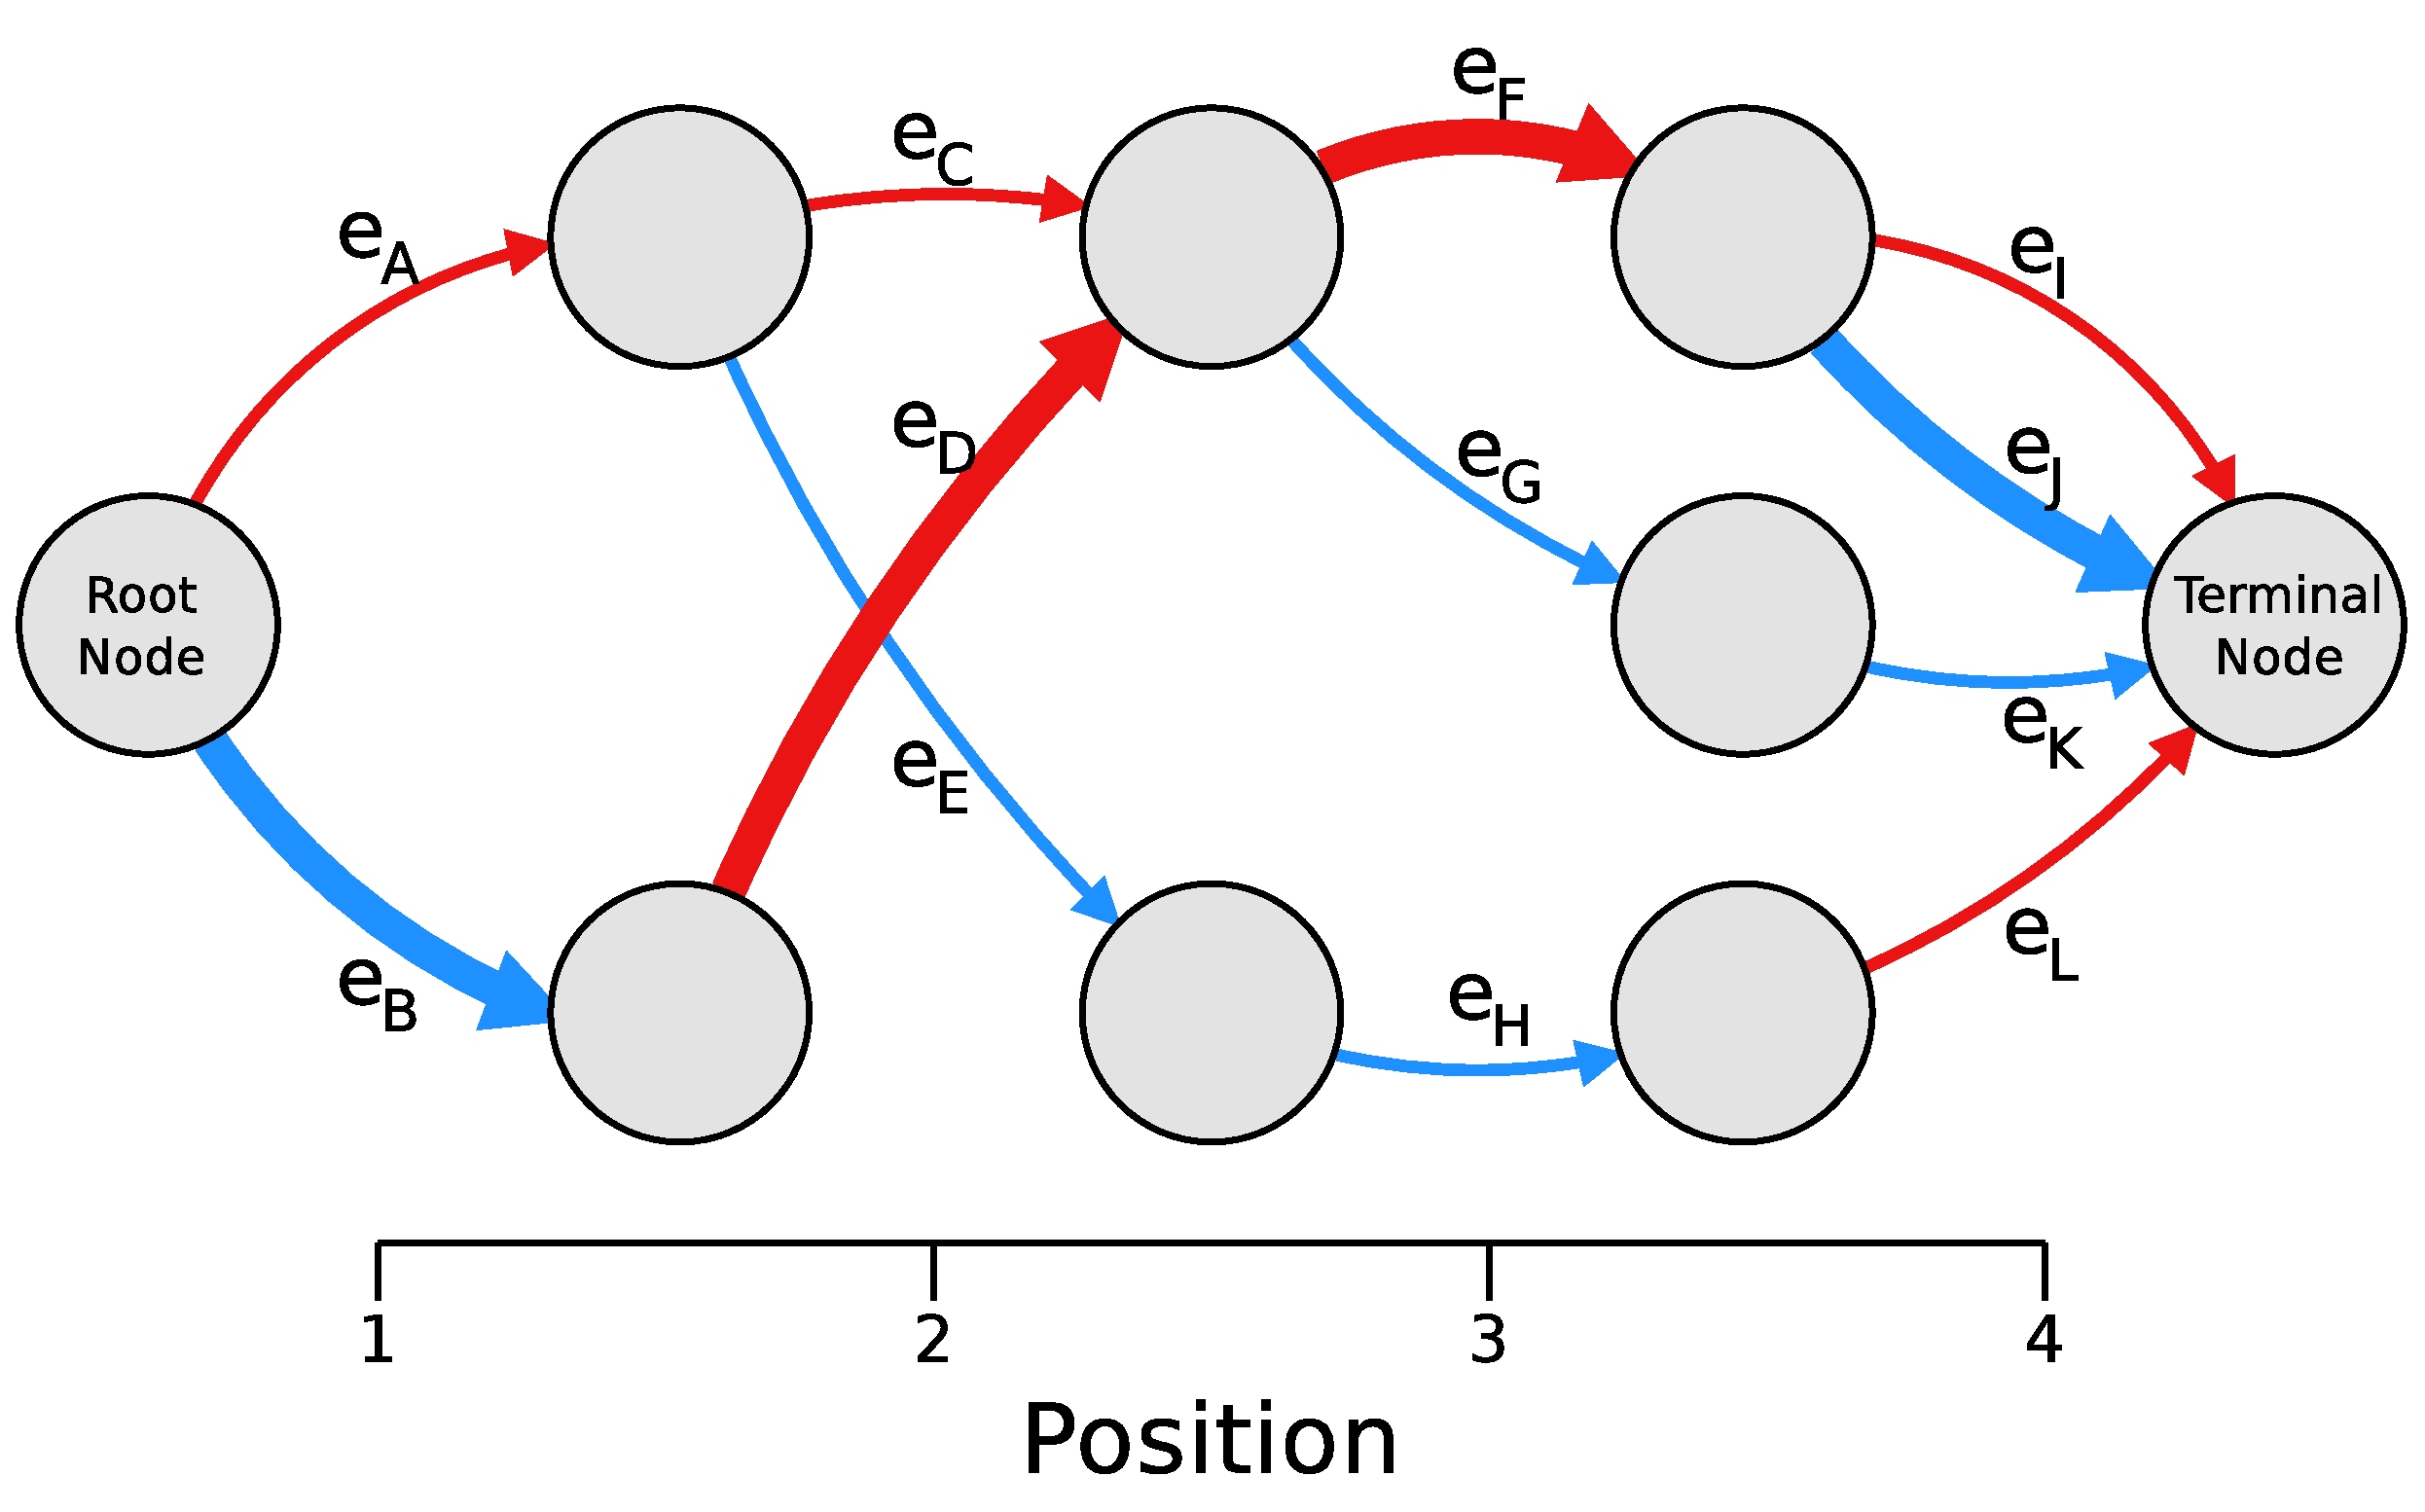
\includegraphics[width=\textwidth]{chap3figs/beagle}
  \end{minipage}
  \caption[The Beagle haplotype model]{\textbf{Left:} Observed haplotypes across four sites. \textbf{Right:} The Beagle haplotype cluster graph that represents these haplotypes. Red edges correspond to the 0 allele and blue correspond to the 1 allele. Each path from the root to terminal node is a haplotype listed in the table. The bold edges denote the path representing the 1001 haplotype.\label{chap3:beaglefig}}
\end{figure}

Beagle initialises all individuals' haplotypes by assigning random phase to heterozygous sites.  It then builds its haplotype graph and calculates the forward variable for each individual, which can then be used to sample a consistent haplotype pair for each individual. The haplotype graph is then rebuilt from these newly sampled haplotypes.  On the final pass the Viterbi algorithm is applied rather than path sampling to obtain final haplotype estimates.  Perhaps the most impressive aspect of Beagle is the speed with which the model converges, ten iterations are used by default and increasing this number yields little improvement in accuracy~\citep{browning2007}.  Whilst the Beagle graph greatly reduces the state space of the HMM, the construction of the graph is somewhat computationally expensive with cost somewhere between linear and quadratic time.  This will limit Beagle's utility for very large samples.
\subsection{HAPI-UR}
The \textbf{HAP}lotype \textbf{I}nfer-ence for \textbf{U}n\textbf{R}elated samples (HAPI-UR)~\citep{williams2012phasing} method is a relatively new phasing method developed with very large samples in mind.  Similar to Beagle and SHAPEIT1 it collapses conditioning haplotypes $H$ into a graph structure which is then used to infer haplotype pairs per individual. The difference between Beagle and HAPI-UR is that the states that this graph represents are no longer bi-allelic configurations but multi-allelic haplotype chunks. 

\vspace{10pt}
\begin{SCfigure}[1][h]
                \centering
    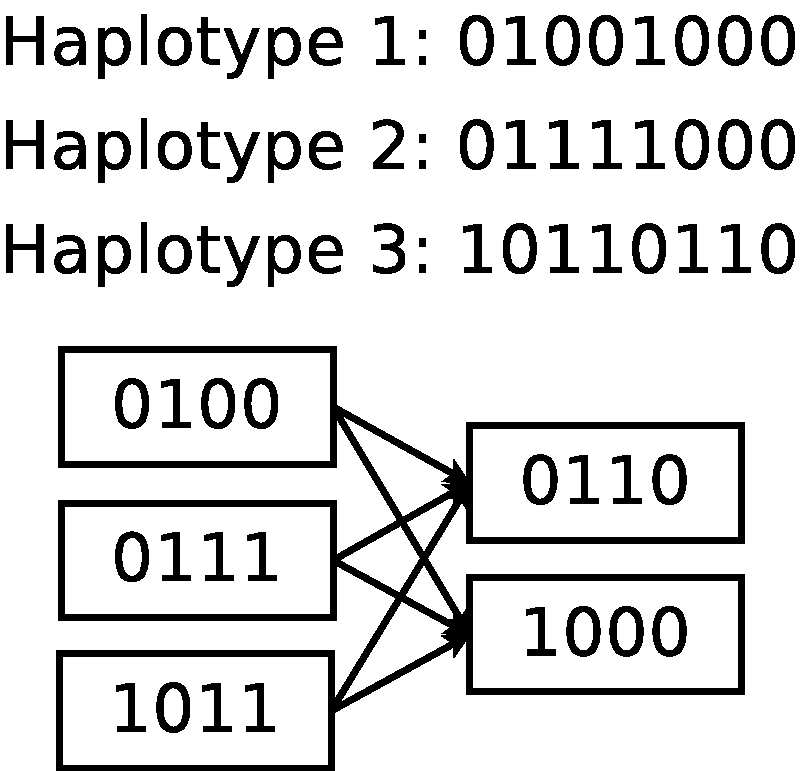
\includegraphics[width=.45\textwidth]{chap3figs/hapiur}
  \caption[The HAPI-UR haplotype model]{The HAPI-UR haplotype graph.  The three conditioning haplotypes are represented in the graph structure pictured below them. All haplotypes are distinct for the first four markers, creating three distinct states.  The last four markers are the same for the first two haplotypes allowing them merge to the same state.  This representation reduces both the state space and the number of locations where transitions can occur. In practice, the length of the segments is allowed to vary.\label{chap3:hapiur}}
\end{SCfigure}

 Figure~\ref{chap3:hapiur} gives a toy example of this graph across eight markers with three observed haplotypes. The markers are split into two segments with three and two states respectively.  This graph not only reduces the statespace but also the number of locations where state transitions can occur.  This graph structure is similar to one used in SHAPEIT1 but with the key difference that the number of markers per segment is allowed to vary within the model. The edges are weighted via modified Li and Stephens model and no mutation events are allowed, so an individual's haplotypes have to exactly match a path through this graph.  This rather rigid model allows very fast inference but comes at some cost in flexibility, new states need to be added to the graph for a single base pair change.  HAPI-UR is currently the fastest algorithm for unrelated individuals, but is less accurate than SHAPEIT2.  The recommended pipeline for HAPI-UR is to run it three times with different seeds, then the outputs from individual runs ``vote'' on the phase at each heterozygous locus. We follow this procedure in our experiments and denote the method as ``HAPI-UR 3X''.
\clearpage
\section{Phasing explicitly related individuals}
The phasing methods described in the previous section infer haplotypes by leveraging linkage disequilibrium, which typically reflects very distant relatedness of an unknown degree between individuals within a sample.  When we deal with explicit pedigrees containing very close relationships, the model we need to use is simpler (at least conceptually). We know a child receives one haplotype from each parent and that we can expect very few recombination crossover events per chromosome, meaning the haplotype a parent \emph{transmits} to a child is a mosaic of that parent's two haplotypes containing very few breaks.  Routines for using parent-child (duo) and mother-father-child (trio) relationships are included in SHAPEIT2, Beagle and HAPI-UR and we describe how these work here.  Routines for complex pedigrees of general structure require more specialised inference machinery, probably the most well known being the Lander-Green algorithm of which we also give an overview.  We also discuss the limitations of each of these approaches.

\subsection{Simple Duo/Trio Phasing}
Given a father-mother-child trio and ignoring crossover events (of which there are only several per chromosome) we only need to consider four haplotypes for the six individuals.  These are the two haplotypes the child receives from its parents (transmitted) and their complements (untransmitted).  Enforcing Mendelian inheritance then constrains the phase at any site that is not heterozygous throughout the pedigree. In the case of SHAPEIT2 this is achieved by placing constraints on its segmented haplotype graph. Beagle performs this by modelling the trio as four independent haplotypes and sampling haplotypes (based on its graph) that are consistent with the trio data~\citep{browning2009unified}. This simple Mendel phasing is relatively easily to integrate with LD based phasing methods, and will result in the same haplotype estimates as the more sophisticated Lander-Green algorithm (described next) in the case of a standalone duo or trio.  

Whilst useful, the duo/trio phasing available in several standard software packages has limitations. It does not elegantly generalise to larger complex pedigrees, such pedigrees could partitioned into small duos and trios but this is sub-optimal.  Consider a nuclear family with five children, it could be partitioned into two duos, but one child would not be able to exploit any parental relationship.  It is uninformative of meiosis, Figure~\ref{chap3:trio} shows a trio with its true underlying haplotypes (left) and those inferred by Mendel phasing (centre), a switch error is induced on the paternal haplotypes due to a crossover event. Crossovers are of course rare so this is not a serious issue unless a researcher wishes to study recombination.  Mendel phasing is also sensitive to genotyping error.  Genotyping errors that cause Mendelian inconsistent genotypes will be flagged as missing in any sensible QC pipeline, for example a site where the mother was AA, the father was AA and the child was BB would be flagged as missing throughout the pedigree.  However not all errors cause Mendelian inconsistency, and if these are left in the data they can induce a switch error throughout the pedigree, see figure~\ref{chap3:trio} right.  

\begin{figure}[h]
\vspace{20pt}
  \begin{center} 
    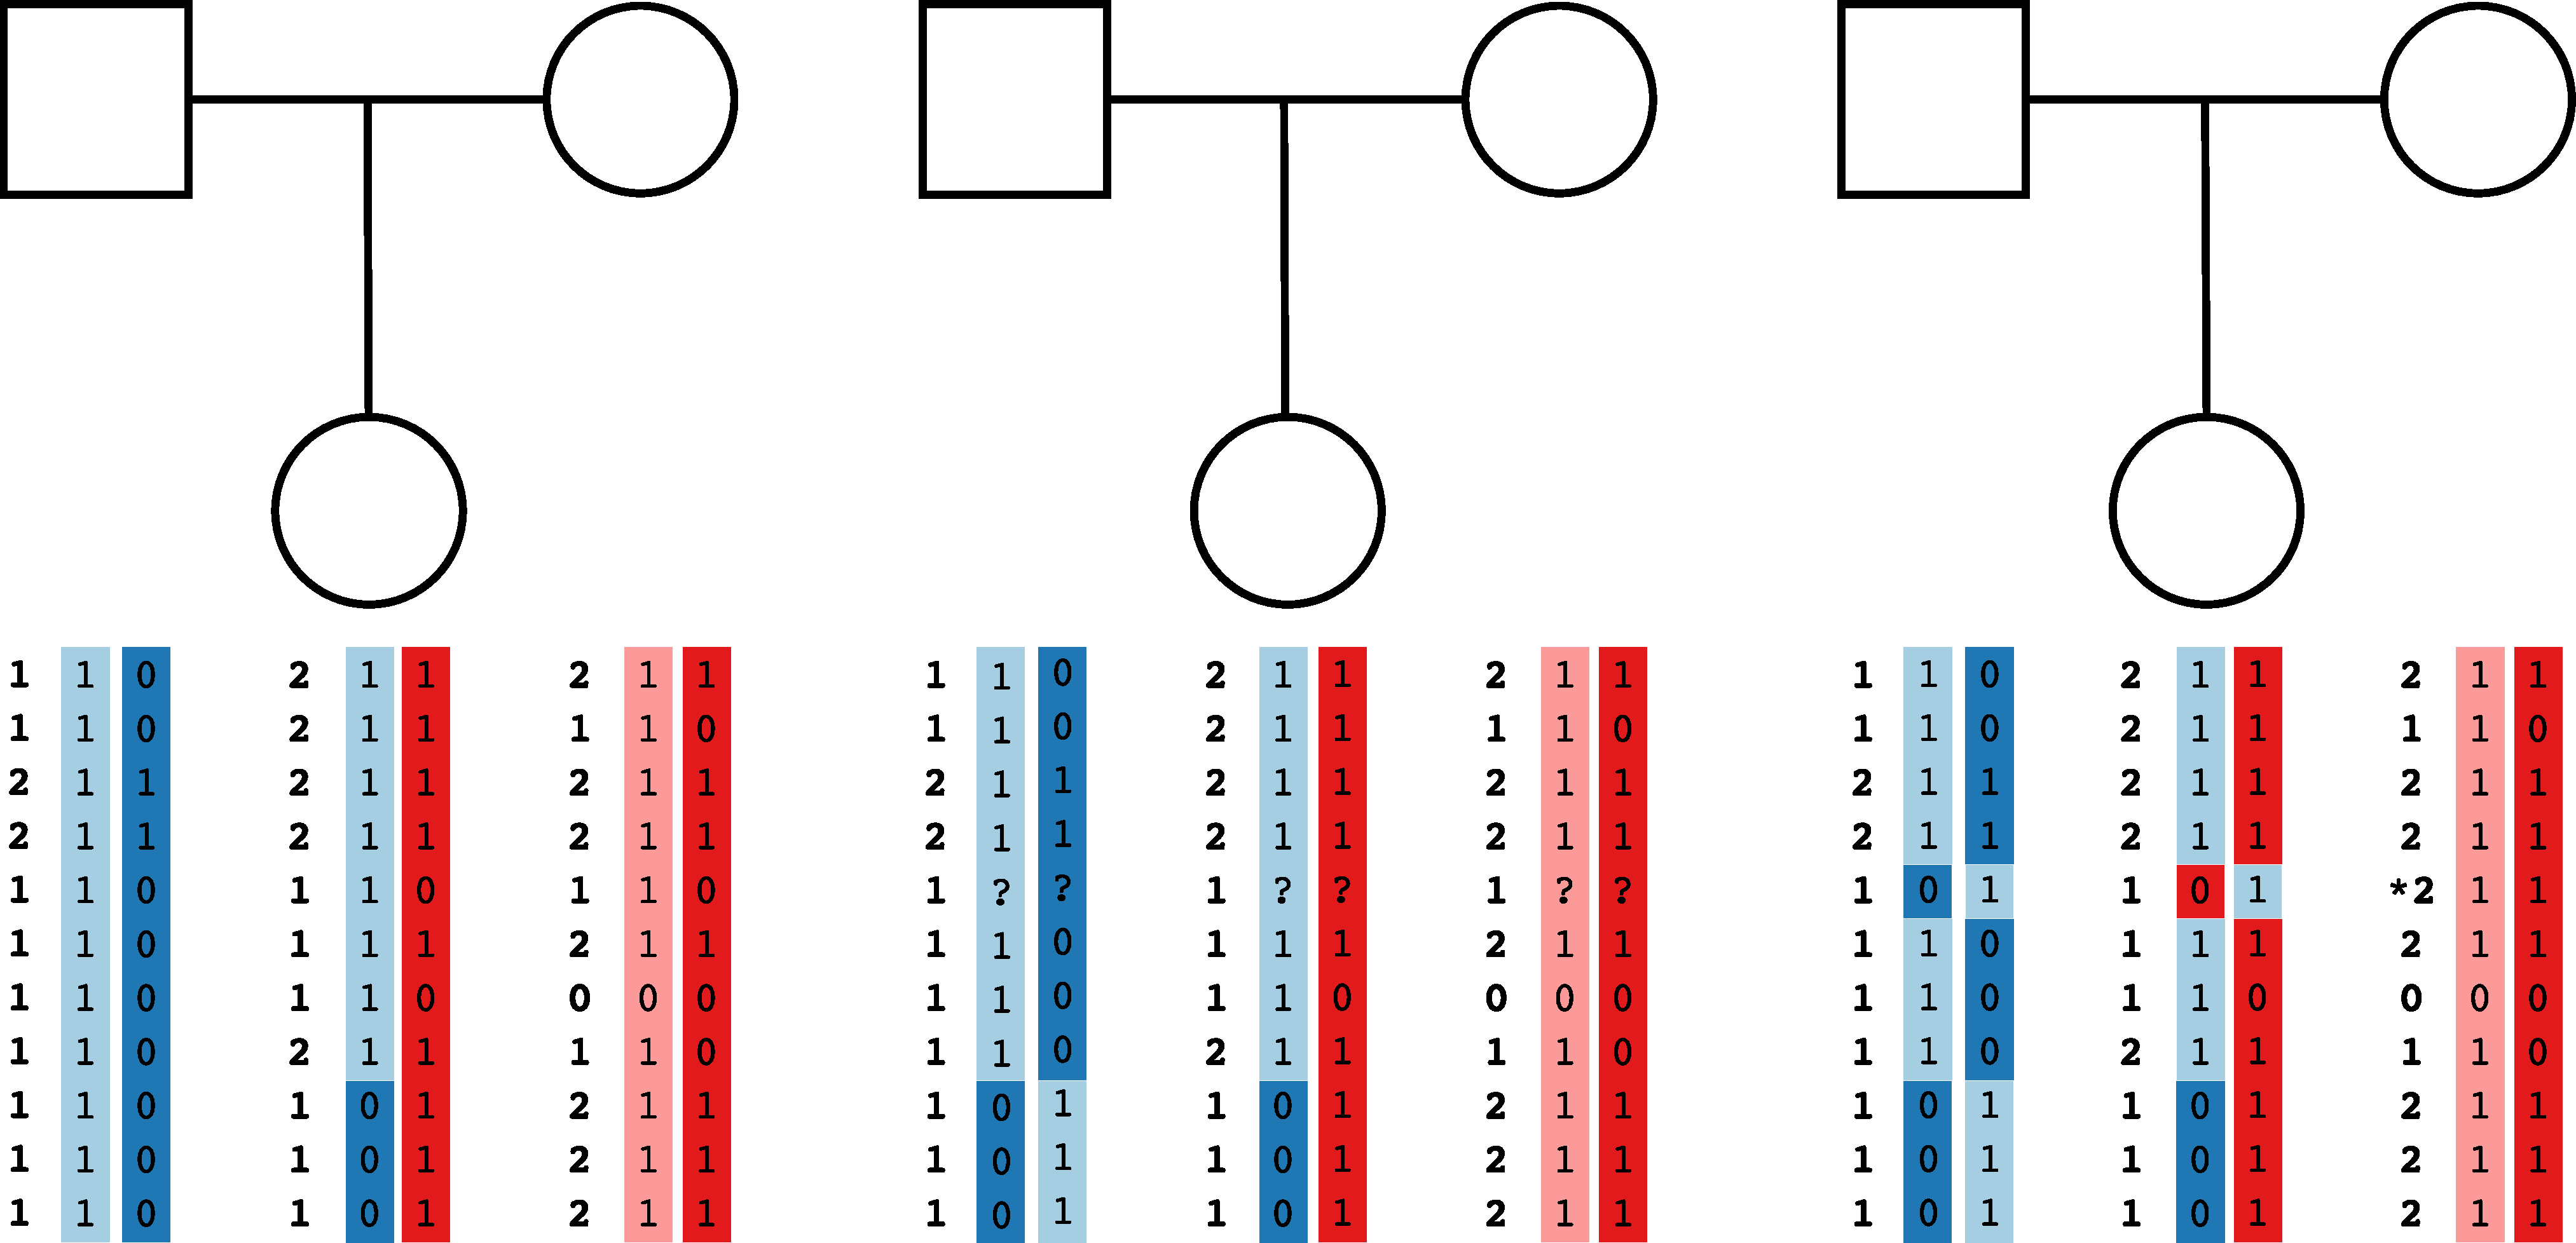
\includegraphics[width=\textwidth]{chap3figs/trio}
    \caption[Father-mother-child trio phasing examples]{Father-mother-child trio phasing examples.  The paternal haplotypes are in light/dark blue and the maternal in light/dark red.  Genotype values are to the left of haplotypes.  \textbf{Left:} True underlying haplotypes, a crossover event has occurred on the paternal meiosis meaning the child's haplotype is a mosaic of the father's two haplotypes. \textbf{Centre:} The haplotypes that will be inferred by phasing with Mendel's rules.  The site that is heterozygous in all three individuals cannot be phased with the pedigree information alone, but will be resolved using LD information from the wider population. The father's haplotypes have been inferred as the transmitted and untransmitted haplotypes (the recombined haplotypes) inducing a switch error.  Since there are very few crossovers per chromosome this is not a serious issue unless we wish to study recombination explicitly.  \textbf{Right:}  A genotyping error has been introduced in the mother (denoted by *) this causes incorrect phasing to propagate to the father and child.  Since the error is still Mendelian consistent, it is difficult to detect.\label{chap3:trio}}
  \end{center} 
\end{figure}
\clearpage
\subsection{The Lander-Green Algorithm}

The simple Mendel phasing rules described in the previous section do not elegantly generalise to situations where there is $>1$ meiosis present in a pedigree since parents transmit different haplotypes to different siblings due to recombination.  The Lander-Green (LG) algorithm~\citep{lander1987} finds the most likely haplotypes for individuals in a pedigree, conditional on the pedigree structure and the individual's genotypes.  The algorithm is computationally expensive, and there have been many clever implementations (and approximations) to improve efficiency~\citep{sobel1996descent,gudbjartsson2000allegro,abecasis2002merlin,lange2013mendel}. We describe a na\"{\i}ve implementation here. 

Given a pedigree with $N_F$ founders and $N_D$ descendants (and hence $N_D$ meioses), there are $2^{2N_D}$ possible patterns of gene flow (which founder haplotype a descendant has inherited) in the pedigree.  Patterns of gene flow can change due to recombination events as we move along the chromosome. Figure~\ref{chap3:landergreen} visualises the gene flow for a three sibling nuclear family with paternal (P), maternal (M) and child (C1-C3) haplotypes. There are two changes in gene flow due to recombinations in first the paternal meiosis (to C2) and then the maternal meiosis (to C3). This process can be modelled as a Markov chain with $2^{2N_D}$ possible states across the chromosome with transition probabilities calculated from the genetic distance between markers and with emission distribution that is a function of allelic frequencies.  

We enumerate each possible inheritance pattern at site $l$ and store them in inheritance vector $V_l$ of length $2N_D$. The $(2i-1)$th position of this vector is 0 if the $i$th non-founder individual received their parents first haplotype and 1 if they received the second.  The $(2i)$th position has the same property but for the maternal chromosome.  The pattern of inheritance can change across the chromosome so we have a sequence of inheritance vectors, $V=\{V_1,\ldots,V_L\}$ .  These vectors are visualised (along with changes due to crossovers) in the bottom row of figure~\ref{chap3:landergreen}.

\begin{figure}
  \begin{center} 
    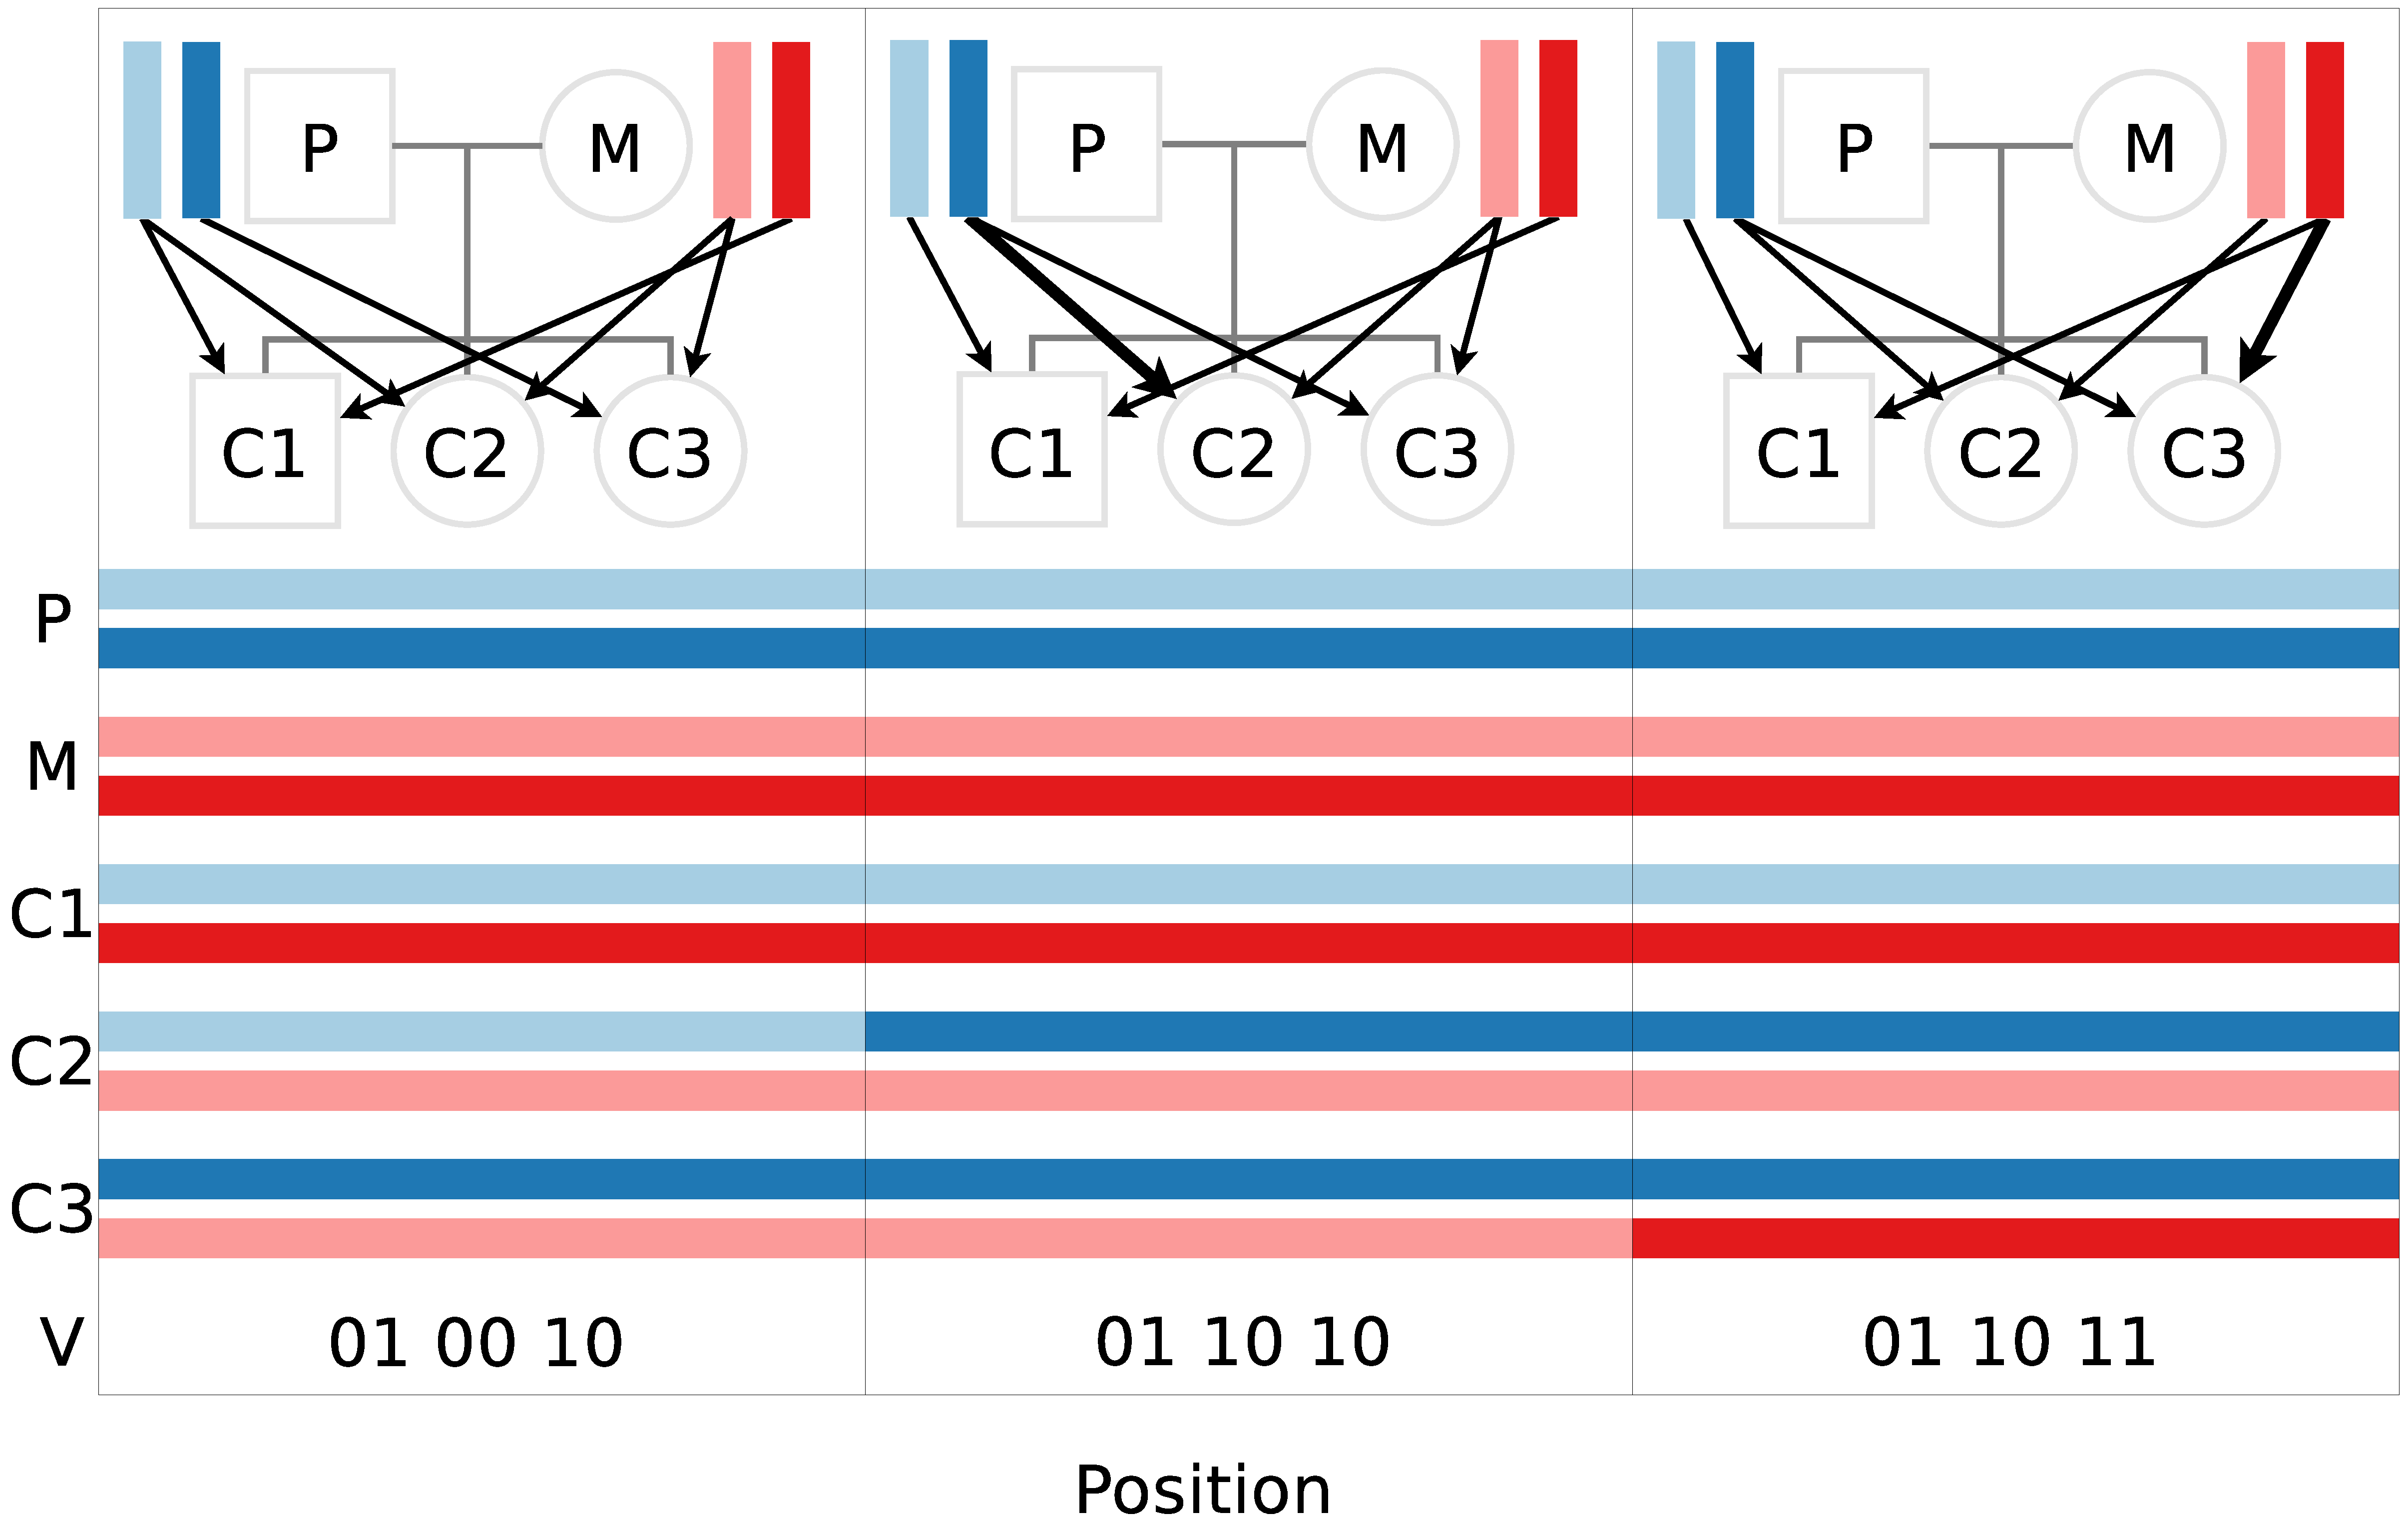
\includegraphics[width=\textwidth]{chap3figs/nuclear_family}
    \caption[The Lander-Green haplotype model]{An example of the Lander-Green Markov process for a three sibling nuclear family.  The paternal (P) chromosomes are in blue and the maternal (M) in red.  Children C1, C2 and C3 receive one (possibly recombined) chromosome from each parent coloured accordingly. The horizontal bars denote the haplotypes of individuals across a genomic region, with the colour of the bar changing when a crossover has occurred on the haplotype received from the parent. The edges in the pedigree diagram indicate the current state of gene flow, with the bold edge indicating a change in inheritance from the previous position. The state $V$ is the binary inheritance vector representing the gene flow pattern at each position.  \label{chap3:landergreen}}
  \end{center} 
\end{figure}
  
\clearpage
The inheritance pattern can change between sites $l$ and $l+1$ according to the transition  matrix $\T_l^{\otimes 2N_D}$, which is calculated by recursively taking the Kronecker product of the matrix
\[ \T_l  = \left[
  \begin{array}{c c}
1 - \rho_l &   \rho_l \\
 \rho_l & 1 - \rho_l  \\
  \end{array}  
\right] \]
with
\[ \T_l^{\otimes n + 1}  = \left[
  \begin{array}{c c}
    (1 - \rho_l)\T^{\otimes n} &  \rho_l\T^{\otimes n} \\
    \rho_l\T^{\otimes n} & (1 - \rho_l)\T^{\otimes n}  \\
  \end{array}  
\right] \]

where $\rho_l$ is the per-generation recombination rate between sites $l$ and $l+1$. The matrix $\T_l^{\otimes 2N_D}$ is then a symmetric $2^{2N_D} \times 2^{2N_D}$ matrix where the diagonal corresponds to 0 crossovers for all meioses.  The transition probability $P(V_{l+1}=k|V_l=k')$ is then the $(k,k')$th entry of $\T_l^{\otimes 2N_D}$.  

We also require the emission distribution which is 
$$ P(G_l|V_l)  = \sum_a \prod_{i=1}^{2N_F} f_{a_i}$$
where $a=[a^1,\ldots,2^{N_F}]$ enumerates every possible set of founder (haploid) alleles that are consistent with $G_l$ and $V_l$, and $f_{a_i}$ is the frequency of allele $a_i$.  

The likelihood for this process is then:
$$L(G) = \sum_V P(V_1) \prod_{l=1}^{L-1} P(V_l|V_{l+1}) \prod_{l=1}^L P(G_l|V_l) $$
 
We can apply the Viterbi algorithm to this likelihood to obtain the most likely sequence of inheritance vectors across a chromosome and then choose the most likely set of alleles from  $a$, for $V_l$. Note that for bi-allelic loci, when at least one individual at site $l$ is homozygous then there is at most one possible $a$ per state. When all individuals are heterozygous there are two equally likely versions of $a$ meaning phase cannot be reliably assigned.

The Mendel phasing rules for duos/trios described at the start of this section are actually a special case of phasing with the LG algorithm.  When there is only one descendant present in a pedigree the emission distributions for each possible gene flow pattern will be equal and since the probability of recombination between markers are typically $\rho_l << 0.5$ there will be no state transitions.  This means that there are four equally likely state paths across the chromosome where the state is just one of the four possible inheritance patterns and is unchanging across the chromosome.  Each path corresponds to a different arbitrary ordering of parental haplotypes.  This is an example of what we will refer to as an \emph{uninformative} meiosis, in that it is uninformative towards recombination events. We define \emph{informative} meioses as those where either grandparents are genotyped or $>2$ siblings are genotyped. Such data allow us to determine crossover events unambiguously.

\subsubsection{Limitations of the LG approach}

\paragraph{Complexity}
A na\"{\i}ve implementation of the LG algorithm must evaluate $2^{2N_D} \times 2^{2N_D}$ possible state transitions between loci giving the algorithm exponential complexity $O(2^{4N_D}L)$. Merlin utilises sparse binary trees to avoid unnecessary calculations such as inheritance patterns that are either impossible (incompatible with observed genotypes) or are equally likely (redundant) making it more efficient than a na\"{\i}ve implementation.  However computation still scales exponentially and pedigrees with say $N_D>30$ non-founders are intractable to analyse.  In practice such large pedigrees can be partitioned for tractable analysis so this issue is largely one of inconvenience.

\paragraph{Sensitivity to genotyping error}
Non-Mendelian genotyping errors that induce switch errors such as that pictured in figure~\ref{chap3:trio} (right) can often only be accommodated via unlikely patterns of recombination with the erroneous marker typically being flanked by two crossover events.   Merlin and other pedigree software provide some functionality to detect probable errors based on these unlikely recombination patterns.  Genotypes at these loci can then be marked as missing throughout a pedigree. However the power to detect errors decreases with pedigree size and is non-existent for parent-child duos and father-mother-child trios.

\paragraph{Resolution of heterozygous sites throughout a pedigree}
Heterozygous founder genotypes where neither haplotype passes through a homozygote descendant cannot be resolved (both haplotypes are equally likely under the LG model).  For research groups applying pre-phasing and imputation pipelines, which are now a standard part of GWAS, this is particularly problematic.  Such incomplete haplotypes cannot be readily used with available imputation software.  Whilst it would be possible to incorporate these haplotype constraints into, say the SHAPEIT2 segmented graph, such functionality would be complicated to implement.

\section{Long-Range Phasing}
 As sample sizes increase, becoming a substantial fraction of the total population (>1\%), the chances of an individual having a recent ancestor in the sample becomes substantial. At any particular location, the chance of two individuals inheriting genetic material from an ancestor $M$ generations ago rapidly becomes small with probability equal to $2^{-2M+1}$, but when common material is inherited it will be a relatively large tract of DNA that is distributed approximately exponentially with mean $100M^{-1}$ centiMorgans~\citep{browning2012identity}.  This sharing of relatively large haplotypes has been referred to as `long-range LD'  \citep{kong2008detection}.

This long range sharing of haplotypes can be exploited to aid haplotype estimation. This idea was first proposed by  \cite{kong2008detection} who made the observation that sampling a large enough fraction of a population (which was possible in the rather unique Icelandic population) will increase the chance that two individuals will share a long region of genetic material IBD. A method was proposed in which `surrogate parents' (IBD sharers) are identified for each individual in a given region of the genome. These surrogate parents allow the haplotypes to be determined with high accuracy using Mendel's rules, effectively as if the true parents had been observed and the family could be phased as a trio.  Kong described a rule based approach and applied it to a large cohort of individuals from Iceland  to produce highly accurate haplotypes. Whilst this was a novel idea, software for general use was not provided.

\subsection{The Systematic Long Range Phasing Algorithm}
Systematic Long Range Phasing (SLRP)\citep{palin2011identity} implements a probabilistic approach to this problem and jointly models the IBD status of all individuals.  The IBD status for each pair of individuals $i$ and $j$ is modelled as a Markov process with hidden state $V^{i,j}_l \in \{1,2,3,4,5\}$ for $l=1\ldots L$ where the states correspond to; 
\begin{enumerate}
\item No IBD
\item IBD between the first two haplotypes
\item IBD between the first haplotype of $i$ and second of $j$
\item IBD between the second haplotype of $i$ and first of $j$ 
\item IBD between the second two haplotypes
\end{enumerate}
We can write the joint distribution of $H$ and $V$ given genotype data $G$ as
\begin{eqnarray*}
  P(H,V|G) &  \propto & P(G|H,V)P(H,V) = P(G|H)P(V|H)P(H) \\
  & = & \prod_{i=1}^N \prod_{l=1}^L \Bigg( P(G_{il}|H_{(2i-1)l},H_{(2i)l}) P(H_{(2i-1)l},H_{(2i)l})\\
&&~~~~~~~~~~~~\times \prod_{j=i+1}^N P(V_l^{i,j}|V_{l-1}^{i,j},H_{(2i-1)l},H_{(2i)l},H_{(2j-1)l},H_{(2j)l})\Bigg)\\
\end{eqnarray*}
The first two terms here are straightforward. SLRP does not model genotyping error so $P(G_{il}|H_{(2i-1)l},H_{(2i)l})$ is just an indicator variable on whether the haplotypes are consistent with the genotype. A flat prior is used for $P(H_{(2i-1)l},H_{(2i)l})$.  

The final term can be factorised to obtain
$$P(V_l^{i,j}|V_{l-1}^{i,j},H_{(2i-1)l},H_{(2i)l},H_{(2j-1)l},H_{(2j)l})\propto P(V_l|V_{l-1}) P(H_{(2i-1)l},H_{(2i)l},H_{(2j-1)l},H_{(2j)l}|V^{i,j}_l)$$
the emission distribution on the haplotypes is simply the product of the four allele frequencies if not in IBD or the product of
 three allele frequencies if the individuals are in IBD. 

The IBD transition probabilities, $P(V_l|V_{l-1})$, come from a continuous time Markov process with rate parameters $\lambda_\textrm{NOIBD}$ for $V=1$ and $\lambda_\textrm{IBD}$ for $V\neq1$ with the constraints that IBD states always transition to the non-IBD state and the non-IBD state transitions to the four IBD states with equal probability.  Hence the transition probabilities between markers $l$ and $l+1$ are 
\[ P(V_{l+1}=k|V_l=k') = \left\{
\begin{array}{c c} 
  e^{\lambda_\textrm{NOIBD} \rho_l}) & k'=1,k = 1 \\
  \frac{1}{4}(1-e^{\lambda_\textrm{NOIBD} \rho_l}) & k'=1,k \neq 1 \\
   e^{\lambda_\textrm{IBD} \rho_l} & k'\neq1,k\neq1,k=k' \\
  1- e^{\lambda_\textrm{IBD}\rho_l} & k'\neq1,k= 1 \\
  0   &  \textrm{otherwise} \\
\end{array}  
\right.\]
SLRP fits this model as a Bayesian network and produces MAP estimates of the both $H$ and $V$.  
%% \[ P(Z_{l+1}=k|Z_l=k')  = \left\{ 
%%   \begin{array}{l l}
%%     \exp(-\frac{\rho_l}{K}) + \frac{1-\exp(\frac{\rho_l}{K})}{K} & \quad k = k'\\
%%     \frac{1-\exp(\frac{\rho_l}{K})}{K} & \quad k \neq k'
%%   \end{array}  \label{chap3:listephentrans}
%%   \right.\]


\subsection{Limitations of Long-Range Phasing}Both the original approach by \cite{kong2008detection} and SLRP  demonstrated very accurate haplotype estimates within IBD regions, but suffer from the problem that phase can only be inferred for genomic regions where IBD sharing is found.  Even in IBD regions, if all individuals are heterozygotes, the phase at that particular locus cannot be inferred.  This is essentially the same problem encountered in pedigree phasing, only partial haplotypes are inferred.  These partial haplotypes could potentially be `filled in' by one of the LD approaches described above, in a manner similar to duo/trio phasing.  Computational complexity is also an issue, SLRP evaluates $N(N-1)/2$ HMMs (every pair of individuals) meaning computational complexity is $O(N^2L)$. This limits the sample sizes that can be tractably analysed.

\section{Integrating extended pedigree information into SHAPEIT2 haplotypes}
\label{chap3:duohmm}
The Lander-Green algorithm is traditionally the method of choice for phasing pedigrees but has several limitations described previously.  The results in the next chapter demonstrate that SHAPEIT2 can in fact phase extended pedigrees extremely accurately, even when completely ignoring any pedigree relationships.  Given this result, there seemed little need to implement a sophisticated LG algorithm within the SHAPEIT2 software itself.  However we would still like to take advantage of the pedigree information for maximum accuracy. 

 We developed a method for analysing SHAPEIT2 haplotypes in a post-hoc fashion when pedigrees are present within a cohort.  First SHAPEIT2 is run ignoring all familial relationships, that is,
 all individuals are treated as if they were unrelated. We then apply a simple HMM to the SHAPEIT2 haplotypes that corrects phasing errors that are inconsistent with pedigree information and to detect subtle genotyping errors. The method focuses on each parent-child duo separately and this circumvents several issues with the Lander-Green algorithm, namely;
\begin{itemize}
\item \emph{complexity}: our HMM has 4 states so there are 16 possible state transitions for each meiotic event, so our method scales as $O(N_DL)$ where $N_D$ is the number of non-founders and $L$ is the number of markers. This compares well to the $O(2^{4N_D}L)$ scaling for a na\"{\i}ve Lander-Green implementation.
\item \emph{heterozygous markers}: markers that are heterozygous throughout a pedigree will be phased via leveraging population haplotypes
\item \emph{sensitivity to genotyping error}: the low computational complexity of the model allows us to accommodate genotype uncertainty
\end{itemize}
We describe the model and several useful applications of it below, we refer to this framework as the duoHMM in later sections of the thesis.
\subsection{The Duo HMM}
Let $p = (p_1, p_2)$ and $c = (c_1, c_2)$ denote a pair of observed (ordered) parental and child haplotypes respectively. Here $p_i = \{p_{i1},\ldots, p_{iL}\}$ denotes the $i$th parental haplotype at the $L$ sites across a chromosome. The same notation is used for the $i$th child haplotype $c_i$. There are four possible patterns of gene flow between the parent and child. The true pattern of gene flow will remain constant over long stretches of a chromosome due to the low rate of recombination in any given meiosis. We use $S_l$ to denote the pattern of gene flow at the $l$th locus, where $S_l = (j,k)$ means that the parents $j$th haplotype and the child's $k$th haplotype are identical by transmission (IBT). Here $j,k \in \{1,2\}$, so there are just four possible transmission patterns, which we denote $A=(1,1), B=(2,1), C=(1,2), D=(2,2)$. The true transmission states $S=\{S_1, \ldots,S_L\}$ are unobserved across each chromosome and we wish to infer them from our imperfect observations of the parental and child haplotypes $p$ and $c$. The intuition behind our approach is that true recombination events and switch errors will cause changes to the pattern of gene flow as we move along a chromosome. Thus we can think of the observed pattern of gene flow as the superposition of two point processes: one with a rate dictated by true recombinations, and a second process with a rate relating to switch errors. Our aim is to deconvolve these two processes to detect the true recombination events and correct switch errors. 

To carry out this inference we have developed an HMM that allows for switch errors in the parental and child haplotypes. We use $\delta_1$ and $\delta_2$ to denote the probability of a switch error on the parental or child haplotypes between two adjacent markers respectively. We also use  $\rho_l$ to denote the probability of a recombination occurring between markers $l$ and $l+1$. Specifically we use $\rho_l = 1 - e^{-r_l}$ where  $r_l$ is the genetic distance between markers $l$ and $l+1$.  We use the genetic distances from the HapMap LD based map \citep{InternationalHapMapConsortium:2005cu} (which are inherently sex averaged) and scale them to the sex-specific genetic lengths from the deCODE 2002 map \citep{kong2002} according to the sex of the parent.

The initial states of the Markov model are given by $P(S_1) = 1/4$. The transition rates on the IBT states $S$ are then given by 
\small
\[ P(S_{l+1}=v|S_l=u) = \left\{ \begin{array}{ll}
    (1-\delta_2) \times \left((1-\delta_1)(1-\rho_l) + \delta_1\rho_l \right)& \mbox{if } (u,v) \in T_1\\
    (1-\delta_2) \times \left((1-\delta_1)\rho_l + \delta_1(1-\rho_l) \right) & \mbox{if } (u,v) \in T_2\\
    \delta_2 \times \left( (1-\delta_1)(1-\rho_l) + \delta_1\rho_l \right) &  \mbox{if } (u,v) \in T_3 \\
    \delta_2 \times \left( (1-\delta_1)\rho_l + \delta_1(1-\rho_l) \right)&  \mbox{if } (u,v) \in T_4   
\end{array} \right. \] 
\normalsize
The sets $T_1, T_2, T_3, T_4$ denote the different types of transition that can occur. The set $T_1 = \{(A,A), (B,B), (C,C), (D,D)\}$ contains the transitions where no change in gene flow occurs. The set $T_2 = \{(A,B), (B,A), (C,D), (D,C)\}$ are the transitions with a change only to  which of the parent's haplotypes are IBT. The set $T_3 = \{(A,C),(B,D),(C,A),(D,B)\}$ are the transitions with change only to which of the child's haplotypes are IBT. The set $T_4 = \{(A,D),(B,C),(C,B),(D,A)\}$ are the transitions with a change to both of child and parental IBT haplotypes. Figure~\ref{fig:duo_hmm_examples} shows examples of how true recombination events and switch errors in parental or child haplotypes lead to changes in the transmission pattern in terms of $T_2$, $T_3$ and $T_4$ events.

We accommodate genotyping error by allowing for errors in the emission part of the HMM. We model the observed haplotypes at the $l$th locus conditional upon the transmission state $S_l$ as follows
\[ P(p_l, c_l | S_l=(j,k)) = \left\{ \begin{array}{ll}
1-\epsilon & \mbox{if } p_{lj}=c_{lk}\\
\epsilon & \mbox{if } p_{lj}\neq c_{lk}\\
\end{array} \right. \] 
Our full model can then be written down as 
\[P(p, c, S) = P(S_1)\prod_{l=1}^{L-1} P(S_{l+1}|S_l) \prod_{l=1}^L P(p_l, c_l | S_l).\]

This method can be applied to any set of estimated haplotypes from parent-child pairs. We run one iteration of the Forward-Backward algorithm, to estimate $\epsilon$, $\delta_1$ and $\delta_2$.   Since there is little uncertainty in the state path this was found to be adequate for convergence. This estimation is carried out on each duo separately. Since the HMM has just four states the computation involved is negligible.

\begin{figure}[p]
 \begin{center} 
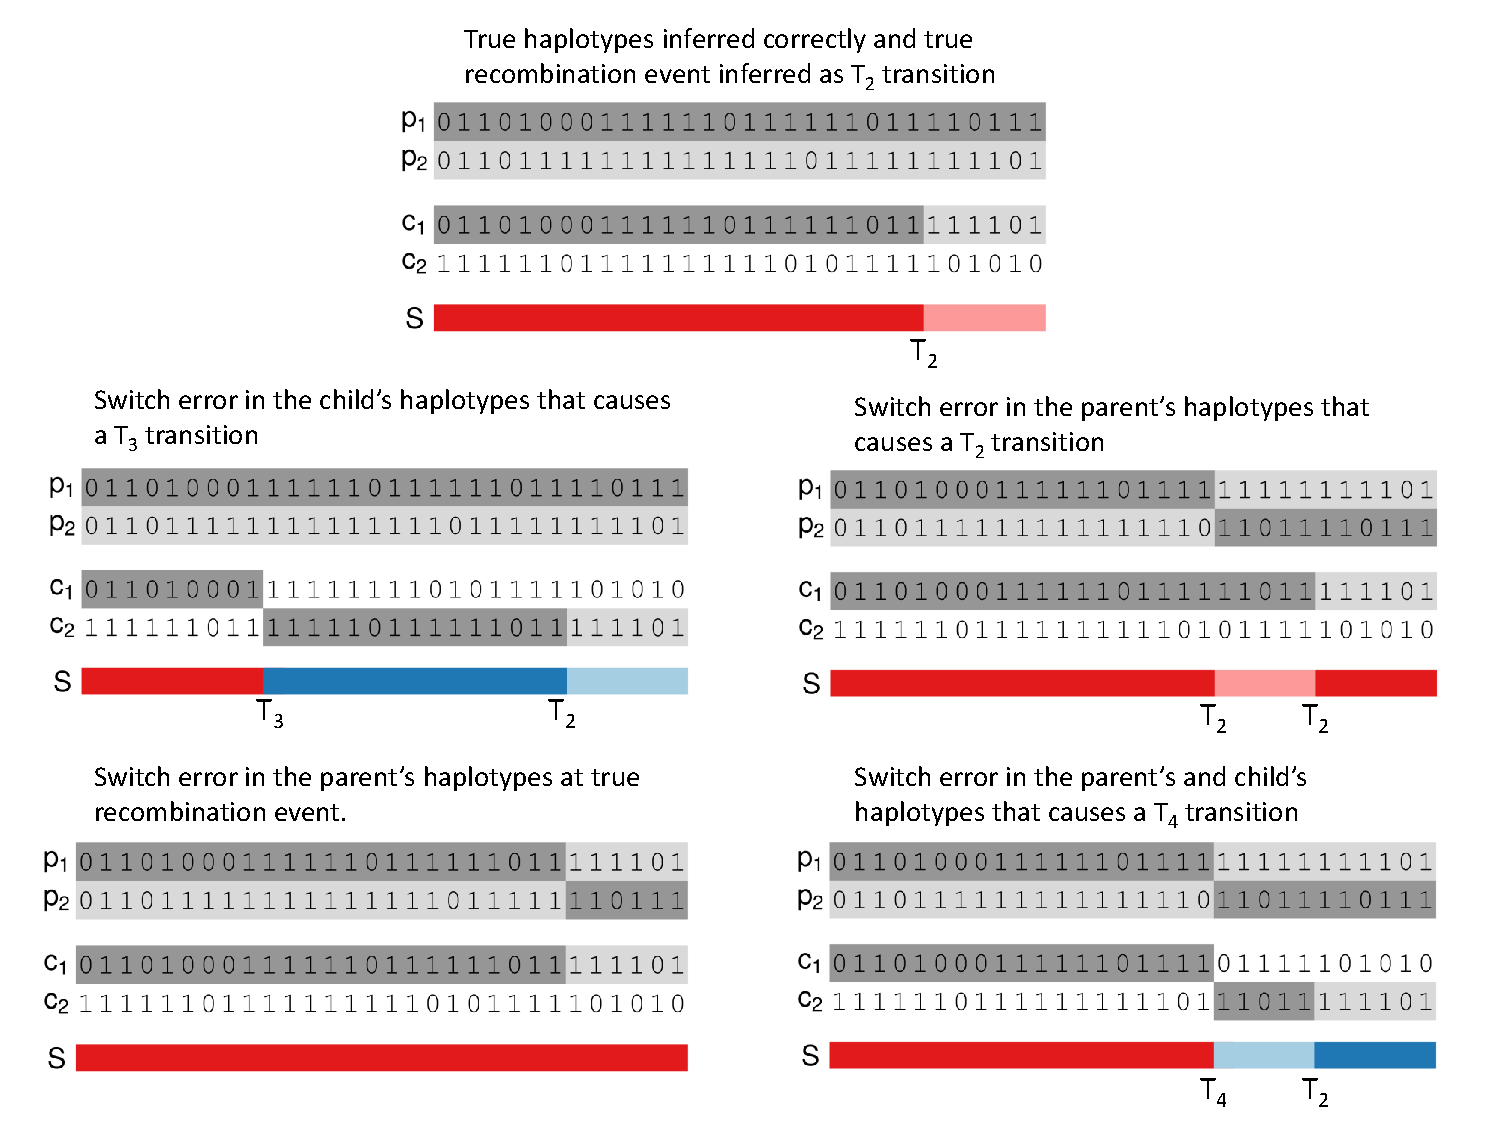
\includegraphics[width=\textwidth]{chap4figs/Fig2}
   \caption[Examples of DuoHMM model]{Examples of inferred haplotypes with true recombination events and switch errors. In each examples $p_1$, $p_2$, $c_1$ and $c_2$ denotes the two parental and child haplotypes and $S$ denotes the pattern of gene flow. \textbf{Top:} Correctly inferred haplotypes in a region of a true  recombination event that causes a $T_2$ transition in the duo HMM. The other 4 examples in the figure add switch errors to these true parental and child haplotypes. \textbf{Middle~left:} addition of a switch error in the child's haplotypes that causes a $T_3$ transition. \textbf{Middle~right:}  addition of a switch error in the parent's haplotypes that causes a $T_2$ transition. \textbf{Bottom~left:} addition of a switch error in the parent's haplotypes at the site of the recombination event that causes the $T_2$ transition to be missed. \textbf{Bottom~right:} addition of a switch error in both the child's and parent's haplotypes at the same position that causes a $T_4$ transition.\label{fig:duo_hmm_examples}}
 \end{center} 
\end{figure}

\subsection{Correcting haplotypes}

We now describe how to use our model to adjust haplotypes so that they are consistent with a given pedigree structure. After estimating parameters, we run the Viterbi algorithm to find the most likely state sequence.  There are sixteen possible state transitions in our model. The eight transitions in the sets $T_3$ and $T_4$ imply a switch error in the child haplotypes, so when we observe one of these transitions in the Viterbi sequence we infer a switch error in the child. The eight transitions in the sets $T_2$ and $T_4$ imply either a switch error or a recombination event in the parental haplotypes. Inferring whether a recombination or a switch error has occurred in the parental haplotypes is difficult. When more than one sibling is present in a pedigree, we can correct probable parental switch errors via identifying the minimum recombinant haplotypes for the family.  When one of the $T_2$ or $T_4$ transitions is present in the same location for the majority of siblings, this is most likely a switch error on the parental haplotypes and they can be corrected accordingly (see  Figure~\ref{fig:correction_example}) for an example of this process). This is not strictly the maximum-likelihood solution, but the minimum-recombinant and maximum likelihood solutions often yield the same result \citep{williams2010rapid}. When we infer a switch error in either a parent or a child we correct the haplotypes by switching the haplotype phase of all loci proceeding the switch error. This procedure is carried out left to right along the sequence. 


\begin{figure}[h]
  \begin{center} 
   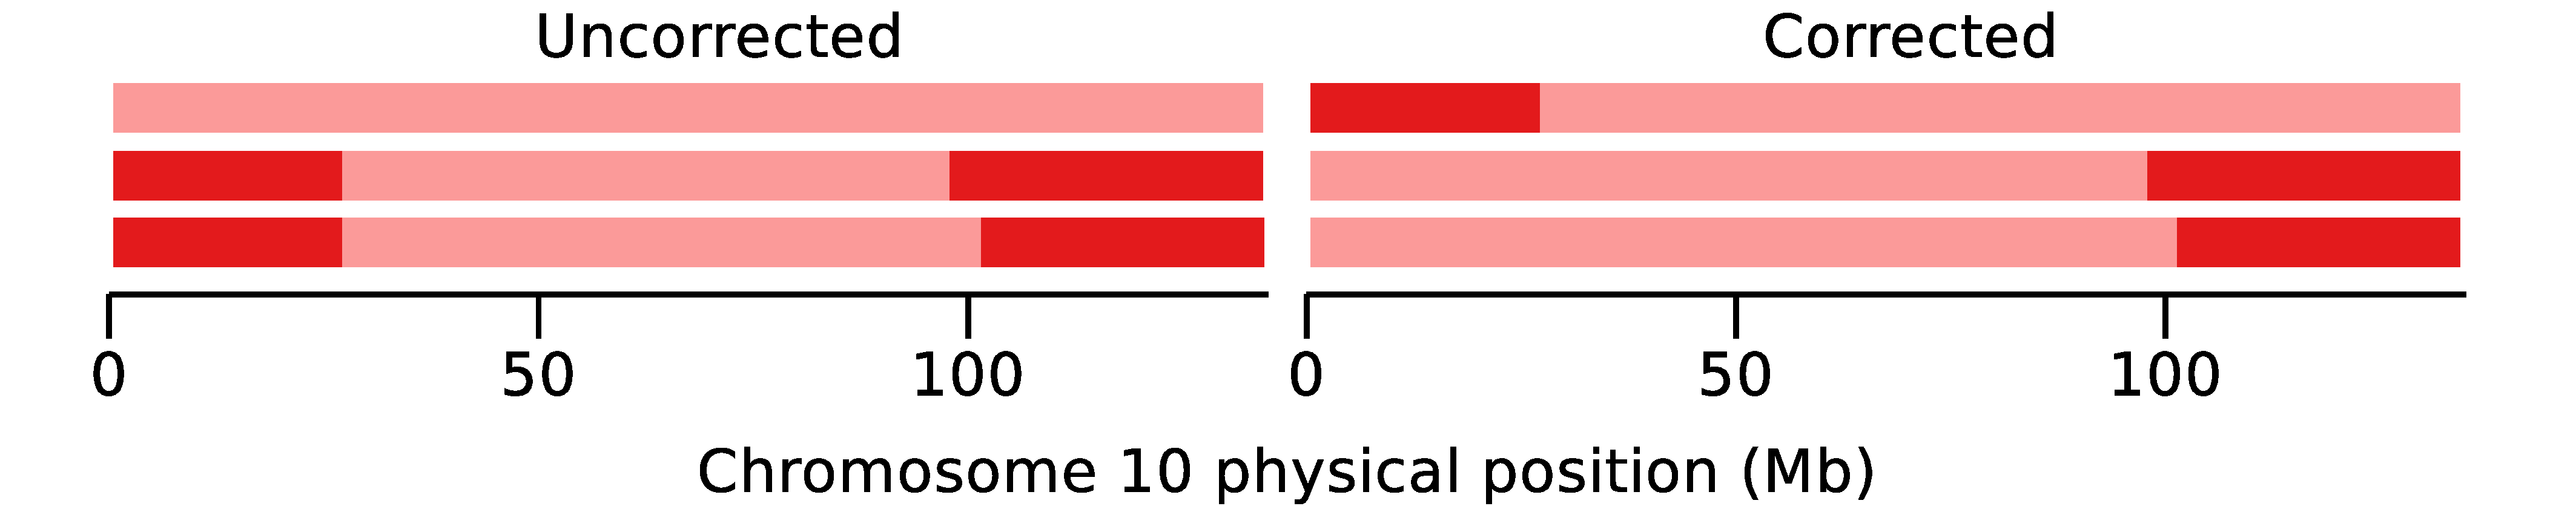
\includegraphics[width=\textwidth]{chap3figs/correction_example}%\vspace{-20pt}    
  \end{center} 
\caption[Haplotype correction example using the DuoHMM]{Haplotype correction example using the DuoHMM. The Duo HMM Viterbi paths for a three father-child duos from a nuclear family (ie. 3 siblings) from the FVG cohort on chromosome 10. The four possible IBT states (A, B, C, D) are shown using colours pale blue, dark blue, light red and dark red respectively (although states A and B do not occur in this example).  The left panel shows the path prior to any corrections, and the right panel after a minimum recombinant correction is applied.  The second and third sibling initially had a $C \rightarrow D$ transition at around 25mb, this is more likely a recombination event in the first child hence the parental haplotypes are switched after this point.  The panel on the right has the corrected haplotypes, the number of recombination events required to explain the observed data has been reduced.\label{fig:correction_example}}
\end{figure}

Corrections are applied sequentially `down' through each pedigree. For example, in a three generation (grandparent-parent-child) pedigree we first apply the method to those duos containing grandparents. Any corrections made to the parents haplotypes are used when processing duos involving those parents and their children. This removes any (detectable) switch errors for individuals that have parents, before their descendants are phased. 

\subsection{Detecting recombination events}
Once all the haplotypes have been corrected the duo HMM is re-run in order to infer recombination events. We do this by calculating the probability of a recombination event between markers. A transition between the parental haplotypes corresponds to either a switch error or a genuine recombination.  A recombination event can only be resolved down to the region between its two flanking heterozygous markers in the parent.  We use $R_{l,l+m}$ to be the indicator variable of a recombination event between heterozygous markers $l$ and $l+m$. We evaluate the posterior probability of such a recombination event as 
\[P(R_{l,l+m}=1|p, c) \propto \sum_{ (u,v)} P(S_l=u,S_{l+m}=v, R_{l,l+m}=1, p,c)\] 
where
\begin{eqnarray*}
P(S_l=u,S_{l+m}=v, R_{l,l+m}=1, p,c) & = & P(p_{1,...,l},c_{1,...,l},S_l=u)  \\
&&\times P(S_{l+m}=v, R_{l,l+m}=1|S_l=u) \\
&& \times P(p_{l+m,...,L},c_{l+m,...,L}|S_{l+m}=v)
\end{eqnarray*}
The first and last probabilities can be calculated from the forward-backward algorithm, and the transition rates that include a recombination event are as follows
\small
\[ P(S_{l+m}=v, R_{l,l+m}=1|S_l=u) = \left\{ \begin{array}{ll}
    (1-\delta_2) \delta_1\rho_l & \mbox{if } (u,v) \in T_1\\
    (1-\delta_2) (1-\delta_1)\rho_l & \mbox{if } (u,v) \in T_2\\
    \delta_2 \delta_1\rho_l  &  \mbox{if } (u,v) \in T_3 \\
    \delta_2 (1-\delta_1)\rho_l &  \mbox{if } (u,v) \in T_4   
\end{array} \right. \] 
\normalsize
Note since the loci between $l$ and $l+m$ are homozygous the emission probability is the same regardless of state, hence we do not require this term in the calculation. A recombination event is inferred when 
\[P(R_{l,l+m}=1|p, c) > t\]
for some threshold $t \in (0,1)$. Rather than calculate these probabilities from SHAPEIT2's best guess haplotypes, we simulate ten haplotypes pairs from SHAPEIT2's diploid graph, repeatedly calculate the recombination probabilities and average the resulting maps. This approach effectively integrates over uncertainty in SHAPEIT2's haplotype estimates.

In the next chapter we compare our method's ability to detect recombination events with the maximum likelihood solution to the Lander-Green algorithm which also will infer crossovers in informative meioses.

\subsection{Detecting genotyping error}
We can also use this model to detect genotyping error at locus $l$, by summing over the posterior probabilities of inheritance states that have inconsistent haplotypes. We use the indicator variable $E_l \in \{1, 0\}$ to denote the presence/absence of a genotyping error at locus $l$ in a duo. Then we have 

$$P(E_l=1|p,c) = \sum_{j=1}^2 \sum_{k=1}^2 I(p_{jl} \neq c_{kl}) P( S_l=(j,k) | p,c )  $$
where $P( S_l=(j,k) | p,c )$ is the posterior probability of transmission pattern $(j,k)$ and can be efficiently calculated from the HMM model. This is the probability of a genotyping error occurring in at least one member of the duo given the observed haplotypes. 

\section{Discussion}

In this chapter we have described a variety of phasing techniques applicable to different types of relatedness present in a sample.  The ideal method would be some form of unified approach that could implicitly exploit the appropriate relationships in a sample.  It would be theoretically possible to accurately assign phase (where possible) using the LG algorithm and a long-range phasing technique, and then place these phasing constraints on the SHAPEIT2 segmented graph.  Unphased sites could then finally be resolved via exploiting LD.  However such an approach would be very complicated to implement.

We have introduced a simple HMM that can integrate extended pedigree information with haplotypes that have been phased using an unrelated method.  This technique enables the detection of recombination events and subtle genotyping errors within pedigrees.  This technique is largely a ``clean-up'' method that relies on the input haplotypes being already quite accurate.

The next chapter extensively evaluates the methods described on both real and simulated data.  We evaluate the ``long-range phasing'' performance of the unrelated methods. We also investigate several strategies for dealing with pedigrees that are part of a larger cohort of unrelated individuals.  We evaluate the potential accuracy improvements of our duoHMM and also contrast its ability to detect crossover events and genotyping error with Merlin's detection capabilities.
